%********************************************************************************
\documentclass{article}[11pt,subeqn]

\title{Assessing Plan B: The Effect of the Morning After Pill on Children and 
Women\footnote{We acknowledge the excellent support and advice of a number of 
members of the Government of Chile who provided extremely useful access to, and 
advice regarding, national databases.  Principally, we thank Rodrigo Alarc\'on S., 
Andr\'es \'Alvarez A., Carlos Arce M\'artinez, Ximena Carrasco and Nicol\'as 
Mu\~n\'oz of the Ministries of Health, Social Development and Education.  Much 
care was taken by all parties to respect all necessary privacy clauses, and data 
analysis was undertaken in line with Law 19.628 of Protection of Private Life 
(\emph{Ley 19.628 de Protecci\'on de la Vida Privada}).  We are grateful to Sonia 
Bhalotra, Lidia Casas, Rachel Cassidy, Julien Labonne, Jeanne Lafortune, Simon 
Quinn, Climent Quintana Domeque, Chris Roth, Margaret Stevens, George
Vega Yon and seminar audiences at ESPE Braga, LAGV Aix en Provence,
the Inter-American Development Bank, the World Bank,
Universidad Adolfo Ib\'a\~nez and the Universidad de Chile for 
useful comments, without implicating them in any remaining shortcomings.  We 
thank Daniela G\'omez P.\ and Katharine Lauderdale for excellent research 
assistance.  Full source code and data are publicly available for inspection 
at \texttt{https://github.com/damiancclarke/morning-after-pill}.}}
\author{Andrea Bentancor\thanks{Universidad Adolfo Ib\'a\~nez.} 
\and Damian Clarke\thanks{Department of Economics, the University of Oxford.  
Contact: damian.clarke@economics.ox.ac.uk}}
\date{\today}


\usepackage{url}
\usepackage{longtable}
\usepackage{booktabs}
\usepackage{rotating}
\usepackage{dcolumn}
\usepackage{color}
\pagecolor{white}
\usepackage{pdfpages}
\usepackage{lastpage}
\usepackage{lscape}
\usepackage{lineno}
\usepackage{setspace}
\usepackage{amsmath}
\usepackage{amssymb}
\usepackage{breqn}
\usepackage{appendix}
\usepackage{natbib}
\usepackage[capposition=top]{floatrow}

\usepackage{epsfig}
\usepackage{epstopdf}
\usepackage{multirow}


\usepackage{wrapfig}
\usepackage{blindtext}

\setlength\topmargin{-0.375in}
\setlength\textheight{8.8in}
\setlength\textwidth{5.8in}
\setlength\oddsidemargin{0.4in}
\setlength\evensidemargin{-0.5in}
\setlength\parindent{0.25in}
\setlength\parskip{0.25in}

\newcommand{\person}{we\ }
\newcommand{\Person}{We\ }

\bibliographystyle{abbrvnat}
\bibpunct{(}{)}{;}{a}{,}{,}

\newcommand\independent{\protect\mathpalette{\protect\independenT}{\perp}}
\def\independenT#1#2{\mathrel{\rlap{$#1#2$}\mkern2mu{#1#2}}}

\usepackage{changepage}
\makeatletter
\newenvironment{chapabstract}{%
    \begin{center}%
      \bfseries Abstract
    \end{center}}%
   {\par}
\makeatother


\newcommand{\teenfolder}{./..}
\newcommand{\biblioinc}{\newpage \bibliography{./References}}
\newcommand{\JELs}{\\ \emph{JEL codes}: J13,J16,J18,I15,O15. \\}

\begin{document}
%\linenumbers
\begin{spacing}{1.4}
\maketitle

%-------------------------------------------------------------------------------
\vspace{-5mm}
\begin{abstract}
We test whether the availability of the emergency contraceptive (``morning 
after'') pill in the absence of legalised abortion can have effects similar to 
those of other large-scale contraceptive reforms. To do so we examine a 
quasi-experimental policy reform occurring in Chile in 2008. Using vital 
statistics covering all births and fetal deaths over the period 2006-2012, we 
show that the availability of the emergency contraceptive pill reduces pregnancy
and early gestation fetal death, which we argue proxies for illegal abortion.
These effects are particularly pronounced among teenagers and young women: point
estimates suggest a 6.7\% reduction in teenage pregnancy and a 2.9\% reduction
for 20-34 year-olds. Our results suggest that in the context of Chile, a country
with among the most restrictive abortion laws in the world, the emergency
contraceptive pill had effects nearly as large as various abortion reforms
observed in other contexts.
\\ \JELs 
\end{abstract}
\vspace{1cm}

\section{Introduction}
Undesired pregnancy---particularly among young and adolescent women---is a
considerable contributor to poor maternal and child outcomes, and to a lack of
intergenerational mobility.  The last half-century has seen a remarkable 
increase in contraceptive technology, with considerable impacts on rates of such
undesired pregnancy and with far-reaching consequences for the social and 
productive structure of modern society. The widespread introduction of the oral 
contraceptive pill has brought with it lower birth rates, delays in childbearing 
and marriage, higher rates of human capital attainment and labour market 
participation for women \citep{Bailey2006,Bailey2009,GoldinKatz2002a,
GoldinKatz2002b}, reductions in the gender wage differential 
\citep{Baileyetal2012}, and, theoretically at least, more empowered women 
\citep{ChiapporiOreffice2008}.  In the long-run, these outcomes have led to 
generations of children less likely to have divorced parents, and more likely to 
live with college educated mothers \citep{OltmansHungerman2012}.

While the contraceptive pill has had a remarkable impact on a woman's capability
to control the timing of her fertility decisions, these treatments require an
expensive ongoing investment, which is difficult or impractical for certain 
groups of women.  In contrast to the rich literature on the effects of the 
contraceptive pill, very little evidence is available regarding the effects of 
post-coital (non-abortive) birth control.  In this paper \person examine the 
effect of fully-subsidised provision of the emergency contraceptive (EC) pill.  
This so called ``morning after pill'' offers an alternative form of 
contraception in cases where other forms were not used or failed during 
intercourse, or in the case of rape.

The scarce existing literature on this topic suggests that the EC pill may have 
had surprisingly little effect on both pregnancy and abortion 
\citep{Grossetal2014,Durrance2013}. Compared to the large body of evidence 
suggesting that contraceptive technologies such as the oral contraceptive and 
legal abortion can have significant and important effects on pregnancy rates, 
empirical studies of the effect of the EC pill have found small or non-existent 
shifts in fertility outcomes despite high rates of use.\footnote{For example, 
the CDC reports that in the United States between 2006 and 2010, 11\% (5.8 
million) women aged between 15 and 44 used the emergency contraceptive pill at 
least once.  Among 20-24 year olds, the rate is even higher, at 23\% 
\citep{Danielsetal2013}.}  However, existing analyses of the effect of the 
EC pill on birth rates have been limited in terms of the contexts 
examined.  Existing quasi-experimental studies in the literature are focused on 
the United States, where abortion is legal, and hence the scope of the EC on 
net birth rates is likely to be limited, especially if abortion and the EC pill
act as substitutable technologies.\footnote{Indeed, this is explicitly 
suggested, although untested, in the economic literature. \citet{Grossetal2014}, 
in one of the few quasi-experimental studies of the EC pill, write a model of 
contraceptive use where use of the EC pill depends on the outside cost of 
abortion. They find small effects in the USA, however state:
     \begin{quote}
     ``This paper studies the effect of EC during a time period in which
     abortion was legal. The effect of EC might be very different [were]
     abortion to be illegal (Bailey, Guldi, \& Hershbein, 2013; Joyce,
     2013).''
     \end{quote}}

However, in many countries and regions, abortion is highly regulated, allowed
in only extreme cases, or even outlawed entirely.  Recent figures suggest that 
only one third of the world's governments currently allow elective abortion or 
abortion for economic or social reasons, with this number being considerably 
lower in developing regions with high rates of fertility \citep{UN2014}.  For 
areas in which abortion is not decriminalised, it is of considerable interest 
to determine whether the arrival of the EC pill in the absence of abortion 
is sufficient to provide similarly remarkable changes in fertility rates as 
those observed with the historical arrival of the first wave of contraceptive 
technologies to other areas.

%In the case of Chile, prior to the 
%availability of the EC pill, abortion was illegal in all circumstances, and 
%clandestine abortions resulting in hospitalisation resulted in incarceration in 
%some cases.\footnote{Chile is one of only seven countries in which abortion is 
%criminalized in all circumstances, including the cases of fetal inviability, 
%risk to the life of the mother, and rape.  [CITE] and numbers.}

A considerable literature on the effect of both the oral contraceptive pill
and abortion, in USA and in other countries, suggests that both may have direct
effects on rates of teen births of around $-4$ to $-9$\%.
Table \ref{TEENtab:lit} provides a summary of the range of estimated effects
found in economic studies of contraceptive reforms.  Although not a comprehensive
meta-analysis, these quasi-experimental studies examining different contexts and
national reforms often find broadly similar effects, suggesting that both
abortion and the oral contraceptive pill alone resulted in significant 
reductions in births. In USA, these estimates suggest that both methods reduce 
childbearing at a young age by about 5.5\% (mean estimate), while in Romania 
and Nepal, the effects are closer to 7\%.  In this paper, we examine whether the 
EC pill alone (where legal abortion is not available) could have effects of
similar magnitude and importance.

In order to examine the effect that the EC pill can have on mothers and children 
when abortion is \emph{not} available, we turn to a particular empirical example.  
We focus on a plausibly exogenous policy decision in Chile which affects a 
woman's access to the fully subsidised emergency contraceptive pill.  We find 
considerable evidence that, at least in the case of Chile, (a country with no 
access to legal abortion in any circumstances\footnote{In Chile abortion is 
illegal in all circumstances, and clandestine abortions resulting in 
hospitalisation result in incarceration in some cases \citep{ShepardCasas2007}.  
Chile is one of only six countries in which abortion is criminalized in all 
circumstances, including the cases of fetal inviability, risk to the life of the 
mother, and rape \citep{UN2014}.}), access to emergency contraception does have 
significant effects on births, and that these effects are concentrated on 
teenagers and young women.  We also find suggestive evidence that EC pill
availability results in a reduction in the likelihood that women recur to
illegal and risky clandestine abortions.  With the arrival of the EC pill, we 
observe a reduction in early term fetal deaths in reform areas, and no similar 
reduction in non-reform areas, while no similar effect is observed for late term 
fetal deaths.  In the case of both births and deaths, the observed effects appear 
to be transversal rather than being centred on more highly educated women.

The reform under examination comes from a series of constitutional challenges 
between 2005-2008, which meant that the introduction of the emergency contraceptive 
pill in Chile was entirely controlled by the Supreme Court and Constitutional 
Tribunal.  Legal challenges resulted in the 2008 finding that it would be illegal 
for all nationally run health centres and hospitals to prescribe the emergency 
contraceptive pill, however that in each of the 346 municipalities of Chile health 
centres were at liberty to do so.  This resulted  in a situation in which a woman's 
access to the EC pill entirely depended upon the decisions taken by her mayor.  Due 
to this reform it is shown that around half the municipalities in Chile made the EC
pill available, while the other half did not.  Using administrative birth data and 
censal population data, we observe each pregnancy in the country leading to a birth
or recorded fetal death, as well as municipal-level birth and fetal death rates.

Using this reform, we estimate the effect that the staggered arrival of the 
emergency contraceptive had on women and children, including its effect on births 
and fetal deaths. The arrival of this new technology is associated with significant 
reductions in these outcomes.  Further, the effects identified are of considerable
magnitude.  It is estimated that among teenage girls, the widespread availability 
of emergency contraception reduces births by around 6.7\%, and reduces rates of early
term fetal death (which we argue may reflect illegal abortion) by approximately 50\%. 
Among older women and the entire country, the reductions in rates of births are more 
moderate, however still quantitatively important.  For example, among 20-34 year-olds,
the emergency contraceptive pill reduces births by an estimated 2.9\%, and the Gross
Fertility Rate in the country is estimated to fall by 3.1\%.
\nocite{Goldin2006, Bailey2011}
\nocite{KearnerLevine2009}
\nocite{Ananatetal2007,ThomasDouglas1996,Levineetal1996}

Naive estimates of the effect of the emergency contraceptive pill on pregnancies,
abortions, and other outcomes, are based on the assumption that the arrival of the
emergency contraceptive to approximately half of the women in the country had no
effect on those women who did not live in areas where the EC pill was available. We
examine the validity of this assumption by comparing women who live `close' to areas
where the EC pill was available to those who live considerably further away.  It is
shown that significant treatment spillovers may occur, and so suggested that naive 
estimates of the effect of the emergency contraceptive pill may significantly 
underestimate the true effect of the expansion of availability in Chile.  We find
the for the EC pill, treatment spillover is a quantitatively important
consideration, and that in some groups, diffusion may exist for anywhere up to 20km
from a treatment location.

This study makes a number of contributions.  Foremost, it is one of the first%
---if not the first---study of the effects of emergency contraception using 
complete microdata on births and deaths at a national scale. It is also the first 
large scale study of which the authors are aware that addresses these questions 
in a country other than the United States.  This is of considerable importance 
given that Chile, the country under study here, does not offer legal abortion, 
and so the emergency contraceptive pill is the first legal mechanism for 
post-coital fertility control.  The context studied here offers lessons on the 
nature of contraceptive reforms, and whether emergency contraceptives in a 
context of high rates of undesired pregnancy and few outside options are 
sufficient to have effects over observed birth rates.
%\footnote{This is not to suggest that \emph{no} post-coital
%contraceptive options exist.  Given the lack of a legal solution, Misoprostol
%accessed on the black market is overwhelmingly to most common method used to
%interrupt undesired pregancies (Casas 2014).}

The results of this study add to the nascent literature on the emergency 
contraceptive pill.  Recent studies such as \citet{Grossetal2014} and 
\citet{Durrance2013} which have been the first to address this question in 
the economic literature have provided evidence to suggest that the effects of 
this technology may be minor.  Here we offer considerable evidence to the 
contrary, suggesting that the expansion in the availability of emergency 
contraceptives may offer important effects in certain countries, with large 
impacts on pregnancy and abortion rates, especially among young women.

%%In what remains of this paper \person first provide background regarding the
%%emergency contraceptive pill, and the reform under study in Chile in section
%%\ref{TEENscn:background}.  Section \ref{TEENscn:Data} discusses the 
%%administrative datasets we will use to assess the effects of the reform, while 
%%\ref{TEENscn:ID} discusses identification and methodology.  In section 
%%\ref{TEENscn:results} \person present results on the contraceptive's effect on 
%%births, abortions and aggregate human capital endowments.  Finally, section 
%%\ref{TEENscn:conclusion} concludes.
  
% > GENERALISE REFORM PART TO DISCUSS FERTILITY IN CHILE
% YUZPE: DIDES 2010 ASK, ONLY 3 OF THE COMUNAS ALLUDE TO ITS USE.
%% IN OFFICIAL DOCUMENTS RELEASED BY THE GOVERNMENT, INCLUDING THEIR GUIDE TO
%% TEEN PREGNANCY, THERE IS NO MENTION OF THIS METHOD.  IN THE PREVAILING LAWS
%% IN BOTH 2006 AND 2012, THERE IS ALSO NO MENTIONS OF THIS METHOD. 
%*******************************************************************************
\section{The History of the Emergency Contraceptive Pill}
\label{TEENscn:background}
\vspace{-5mm}
\subsection{The Emergency Contraceptive Pill}
The emergency contraceptive pill is a hormonal treatment which can be used 
within 5 days of an unprotected sexual relationship to reduce the probability
of conception.  There are a number of alternative types of emergency 
contraceptive pills, however principally these are composed of doses of the 
progestin levonogestrel, or a combined dose of estrogen and progestin. 
Typically these are taken as a single pill or two pills in a 12 hour period
\citep{vonHertzenetal2002}, however similar doses of hormones can be obtained 
by combining normal birth control pills \citep{Ellersonetal1998}.  

This form of contraception has been shown to be relatively effective at 
avoiding undesired pregnancy.  Estimates of around 75\%-85\% effectiveness 
based on typical usage are common, depending upon the method of emergency 
contraception used.\footnote{The WHO's \citet{WHO1998}, for example suggests 
that a levonogestrel routine reduces pregnancy rates by 85\%, with a 95\% 
confidence interval of 74-93\%.}  The success of these treatments is dependent
upon the delay between intercourse and taking the drug, so widespread---or at 
least quickly available---access is important in reducing undesired pregnancies.
While most effective when taken within 12 hours after intercourse, 
effectiveness can continue when taken within as much as 120 hours
\citep{vonHertzenetal2002}.

The emergency contraceptive pill is not an abortive agent, but rather is a 
`postcoital contraceptive' which acts to prevent ovulation 
\citep{Novikovaetal2007, Noeetal2011}. This contraceptive method has been of 
clinical interest since at least the late 1960s \citep{Demers1971}, however 
access to these methods, either by prescription or over the counter, is still 
not universal.  The fact that emergency contraception is non-abortive has 
meant that it is available in many countries in which abortion is absolutely 
prohibited, or prohibited in all cases except where concerns for maternal 
survival exist.  Some countries have made the EC pill available as early as 
the mid-1980s \citep{UKFPA2006}, while many more countries have legalised 
the EC pill during the last decade.

\subsection{The History of EC Pill in Chile}
\label{TEENsscn:Chile}
The introduction of the emergency contraceptive pill in Chile has followed 
a complicated path, with early legislation frequently blocked by conservative 
groups in office and in civil society.\footnote{The Chilean political 
framework is marked by a strong conservative axis, and a constitution which 
favours the maintenance of the status quo in economic and social policies.  
This has been the case since the return to democracy in 1990, with an 
alliance of right wing parties (and some members of the presiding left wing 
coalition) who have ``resisted more liberal changes in the poorly named value 
judgements''  (\citet{CasasBecerra2008}, p.6, author's translation.)}  While 
initial discussions and administrative inquiries took place in 2001, it was 
not until 2005 that significant advances in legislature were made. In 
December of this year the Chilean Supreme Court determined that the Institute 
of Public Health---the pharmaceutical regularity body of Chile---was 
\emph{not} acting unconstitutionally by approving the provision of an 
emergency contraceptive drug on the pharmaceutical register.  However, this 
finding was quickly challenged by detractors, with cases presented before 
ordinary and Constitutional Tribunals \citep{CasasBecerra2008}.

These tribunals were followed by a number of years' worth of legislations and
litigations, which resulted in sporadic availability of the emergency
contraceptive pill, occasionaly freely available from state clinics or by
purchase in private pharmacies. However, these were generally short-lived and
emergency contraception was not consistently stocked, with both political and
economic ramifications for groups providing access to the EC pill.\footnote{For
example, the subsecretary of health was removed from cabinet due to his
announcement in 2005 that emergency contraception would be available to all
women who sought it.}  Details regarding this intervening process and laws
passed by parliament theoretically requiring the provision of emergency
contraception are discussed more fully in the online appendix to this paper.

The period of interest for this study follows a decision taken by the Chilean
Constitional Tribunal in 2008.  This finding, responding to a demand placed by
36 parlamentary deputies in 2006, made it expressly illegal for the centralised
health system to distribute the emergency contraceptive.  This requirement held
for all centres under direct administration of the national Ministry of Health,
but, fundamentally, provided all municipal-level centres and hospitals the 
freedom to distribute the EC pill.  Given that these centres are administered by 
the mayor of each municipality (or \emph{comuna}), the availability in each 
municipality was entirely under the control of the mayor \citep{Didesetal2011,
Didesetal2010,Didesetal2009}.\footnote{Of the 346 municipalities in Chile, 320
have their own health systems, while the remaining 26 depend entirely upon the
Ministry of Health.  These 320 municipalities make up 94\% of the population 
of Chile.  Municipal health centres make up the majority of health centres in 
Chile.  Of the 2501 registered health centres and hospitals, 2049 are under the
control of municipalities \citep{DEIS2013}.}  This resulted in a situation in
which around half of the municipalities in Chile distributed the EC
pill freely, while the remaining half refused to distribute it, or to 
distribute it only in a very restrictive set of circumstances.  At the level
of the woman, her municipality's treatment status was essentially exogenously
determined, being based on the whim of the mayor or representative public 
health bodies in her area of residence.  We provide further discussion of the
mayor and municipality characteristics and EC provision in section 
\ref{TEENscn:ID}.  This idiosyncratic policy environment endured for 
approximately four years, until a law was passed mandating that the emergency 
contraceptive pill must be available to all women who request it.  This new 
law became operational in May of 2013.

The Chilean context is one in which emergency contraception may be expected to
have particularly important effects on pregnancy and maternal health.  Abortion
is entirely illegal in Chile, meaning that in the absence of emergency 
contraception, undesired or accidental pregnancies must either be taken to 
term, or a woman must risk undertaking a dangerous and illegal clandestine
abortion \citep{ShepardCasas2007}.  Figures on the frequency and method of 
clandestine abortion are unclear, however \citet{ShepardCasas2007} suggest that
the primary method is by taking the abortive drug misoprostol, which can be
legally prescribed for treatment of ulcers.  However, the cost of accessing 
this drug without prescription is high.  Dated (2007) figures suggest prices
of 38,000-50,000 Chilean pesos, or around one third of the minimum monthly wage
at this time.  Further discussion related to the contraceptive environment in 
Chile preceding and posterior to the reform are available in online appendix B.  

%--------------------------------------------------------------------------------
\section{Data}
\label{TEENscn:Data}
Population data from Chile comes from two main sources. The first is vital 
statistics data, which records all births and fetal deaths, and is provided by 
the Ministry of Health of the Government of Chile (MINSAL). This data provides 
microdata records covering greater than 99\% of all births and fetal deaths 
reported in aggregate data in the country \citep{Bharadwajetal2013}. Each entry 
records the occurrence of a birth or fetal death, characteristics of the mother 
(and if present the father) including her age, education, and muncipality of 
residence, as well as a number of charactersitics of the birth (including 
birthweight, gender, gestation and birth order) or the fetal death (weeks of 
gestation, birth order, cause of death). These data have been collected and 
reported in Chile since 1982, and, at the time of writing, are publicly 
available up to the year 2012. These vital statistics data for birth and
fetal deaths thus provide data on all pregnant women in the country who either 
give live birth, have a birth leading to fetal death or who miscarry in any 
hospital in the country.

Data on all women of reproductive age comes from the National Institute of 
Statistics of Chile (INE). The INE provides estimates of the number of women 
of each age living in each municipality in each year. These estimates are based 
on the decennial census, as well as net migration each year, and vital 
statistics on all births and deaths occurring to residents in the municipality 
(Instituto Nacional de Estadst\'icas, 2014). These two sources of data provide 
information on the number of women of fertile age living in each municipality, 
and the number of women pregnant (where pregnancy leads to a birth or observed
fetal death) in each municipality during the time period of interest. They can
be merged at the level of the municipality, resulting in counts of total number
of births and women, and also the calculation of municipality-level rates of
pregnancy (births/total women), and fetal deaths (deaths/total births).  We
provide additional details regarding the vital statistics and population data
and their structure and matching in the online appendices provided with this
paper.

This results in a total sample of 1,605,300 births and 13,063 fetal deaths
ocurring between 2006 and 2012 (inclusive).  The number of births per year in 
Chile has remained relatively stable over the last decade.  Figure
\ref{TEENfig:BirthDeath} displays total births, along with total fetal deaths
during the period under study.  Total births vary between around 220,000-%
250,000 per year, while total fetal deaths recorded in the Ministry of Health
data (all fetal deaths occurring in any hospital or clinic in Chile), vary
between 1700 and 2100.

Our measure for the EC pill is a binary variable which records whether the 
emergency contraceptive was freely available to a woman upon request at her 
municipal health centre in the year before her birth outcome is observed.  We
consult two sources to collect data on EC pill availability.  First, in each of 
2009, 2010 and 2011 an independent survey was conducted, asking health care 
workers from each municipality whether they were able to prescribe the EC pill
\citep{Didesetal2009,Didesetal2010,Didesetal2011}. This should 
directly reflect the decision by each mayor regarding whether his or her
municipality could prescribe the EC pill after the 2008 Constitutional ruling.  
In each case, healthcare representatives were also asked to list the circumstances 
in which they could prescribe the EC pill.  All municipalities which reported that
they could prescribe the EC pill freely to women were recorded as treated, while 
all others were recorded as untreated.\footnote{A small number of 
municipalities reported that they could prescribe the emergency contraceptive, 
however that this was only following cases of rape.  These municipalities were 
classed as \emph{un}treated given the lack of widespread availability.
Similarly, a small number of municipal health centres could not be reached
or refused to answer in each year \citep{Didesetal2009,Didesetal2010,
Didesetal2011}. These municipalities were not included in the analysis.}
Secondly, the Ministry of Health has made available administrative data on
all EC pill requests and dispursements at municipality clinics and hospitals.
This allows us to determine the veracity of the survey data discussed
above, while also providing concrete numbers regarding the use of the emergency 
contraceptive pill following the reform of interest.  However, we do not
use EC pill disbursements as the main measure of treatment.  We focus on
reported availability, given that disbursements are endogenous, and
jointly determined by demand as well as supply.\footnote{However, when we
define EC pill municipalities based on disbursements rather than reported
willingness to prescribe, we find effect sizes which are largely similar.
These results are presented in online appendix tables.}

In total, 280 of Chile's 346 municipalities report being able to prescribe the 
EC pill in at least one year after the 2008 Tribunal result (see table 
\ref{TEENtab:SumStats}). Figure \ref{TEENfig:Pilltime} displays the quantity
of municipalities reporting EC pill disbursements over time.  Here, the number
of prescribers increases over time in line with greater awareness of the legality 
of distributing the emergency contraceptive pill.  While less than half of all
municipalities report EC pill availability in 2009, this has increased to around
two thirds by 2011. Official records of EC pill prescriptions suggest reasonably
large fluctuations over time.  While nearly 8000 women were reported as 
requesting the EC pill in 2009, this fell to slightly under 4000 the following
year.  Recent figures suggest that this number has been stable at around 6000-%
7000 requests in 2011-2013 (the most recent two years have been omitted from
this study, and from graphical output, given that official birth records for
2013 are not yet finalised).  Figure \ref{TEENfig:PillGeo} displays
the geographic variation of EC pill availabilitly.  This suggests that the
EC pill is available in all parts of the country. With the exception of the
large and very sparsely populated southern region of the country (the 
10\textsuperscript{th} region) which has no municipal health centres, no 
obvious spatial patterns exist.

\Person examine fetal deaths as a manner to proxy illegal abortion.  While it 
is certainly not the case that all (or even the majority) of fetal deaths 
observed in administrative data are results of abortive drugs, there is some
evidence that these are the result of abortion in some cases, although they are 
recorded in a number of different ways in official figures to avoid criminal 
charges against women \citep{ShepardCasas2007}.  To avoid concerns that 
reductions in fetal deaths may be simply due to greater investments in public
health, \person examine a number of subgroups of interest.  Firstly \person focus 
on deaths occurring between 1-20 weeks of gestation, as this is the period in 
which nearly all abortions are conducted.  Secondly, \person remove deaths which,
based on their ICD code,\footnote{The ICD refers to the International 
Classification of Disease, and refers to a set of standardised codes by which
deaths can be classified.  All deaths in the vital statistics data report this 
code, (the ICD-10).} are clearly not related to abortion, such as those due to 
congenital malformations, deformations and chromosomal abnormalities.  By
using this methodology, a clear validity check exists by comparing reductions
in fetal deaths during 1-20 weeks (which may represent abortions and should
respond to the EC pill), to those occurring from week 21 and above,
which should be largely or entirely unaffected by emergency contraceptive
availability.

Full summary statistics are provided in Table \ref{TEENtab:SumStats}.  These
statistics are subdivided by whether or not the municipality reports having
the EC pill available in
a given year.  We observe some differences between EC pill and non-EC pill
municipalities, such as higher education and health spending in pill 
municipalities.  However, this is largely due to the fact that all years in which
the EC pill was observed occur after 2008 while non-EC pill status is observed over
the entire time period under study.  In order to test this more formally, in
table \ref{TEENtab:pillchoice} each municipality's EC pill status is regressed
on all observed municipality characteristics, mayor characteristics, as well as 
year and region fixed effects.  Unlike the raw summary statistics, this table 
suggests that those municipalities where the EC pill was prescribed do not look
remarkably different to areas where the EC was not prescribed, with two 
exceptions.  Of the observed time varying controls, differences (at a 5\% level)
are observed along the conservativeness of the mayor's party (which is negatively 
related to EC pill status), and by the degree to which condoms are also used in 
the region (which is positively related to EC pill availability).  As we discuss 
later in the paper, we address concerns that municipalities which do and do not 
prescribe the EC pill may differ in a way which threatens identification in a 
number of ways.  Firstly, we estimate full event studies to examine the 
plausibility of parallel trends, secondly, we weight using inverse-propensity 
scores, and thirdly, we include these time-varying controls in our regressions.

Longer time-series trends of the number of pregnancies in Chile are presented
in figures \ref{TEENfig:Trend1519} (births to 15-19 year old mothers) and 
\ref{TEENfig:Trend2034} (for 20-34 year olds).  These figures display the counts 
of total numbers of pregnancies, split by whether or not the municipality 
reported giving the EC pill in 2010.  While there are year-by-year fluctuations, 
from 2004 onwards there is an increasing trend in the absolute number of 
pregnancies in both age groups.  This tendency reverts following the availability 
of the EC pill in municipal health centres.  While this reversion is seen in the 
whole country, it is extremely sharp in municipalities which report that the 
EC pill was available when requested by women.  In the following sections, we
examine this effect econometrically.

%********************************************************************************
\section{Methodology}
\label{TEENscn:ID}
We take advantage of the quasi-experimental nature of the expansion of the 
availability of the EC pill to women in different municipalities in Chile.
Municipality $j$ in year $t$ is considered as treated if public health centres
report that the EC pill is available upon request.  Municipal-level birth
rates $BirthRate_{jt}$ are regressed on the availability of the EC pill
($ECpill_{jt}$) in the preceding year:
\begin{equation}
 \label{TEENeqn:pill}
BirthRate_{jt} = \alpha + \delta\cdot \mathbb{I}\{ECpill_{jt-1}\} + \phi_t +
  \eta_j + \eta_j\cdot t + \bm{X}_{jt-1}\bm{\gamma} + \varepsilon_{jt}.
\end{equation}
In (\ref{TEENeqn:pill}), full municipality and year fixed effects are included,
and municipality-specific time trends are allowed.  In our main specification,
each municipality is weighted by its population of fertile-aged women, although
unweighted results are also estimated. Standard errors are clustered by
municipality.  The identifying variation in availability of the EC pill is by
municipality and year.  Prior to the legal reform the EC pill was unavailable to
all women, while following the reform the EC pill was available to those women
living in municipalities where the mayor did not restrict access.\footnote{%
Prescribing the EC pill in a given year after the reform does not imply that
municipalities necessarily prescribe the EC pill in the years following.  For
example, in some cases municipalities switched from 0 (pre-reform), to 1 (during
reform), back to 0 (during reform), and then to 1 definitively (post-reform)
after the EC pill was made legal in the whole country in 2013. Our identification
strategy takes advantage of this switching, given that $ECpill_{jt}$ varies by
municipality and time.}  This provides a flexible difference-in-differences
(hereafter diff-in-diff) framework, and allows us to causally estimate the effect
of the EC pill if we believe that typical diff-in-diff assumptions hold.  Namely,
we require that unobserved components $\varepsilon_{jt}$ in the above
specification evolve similarly over time in the treated and untreated
municipalities.

Given the geographically disperse, and, as discussed in previous sections,
plausibly exogenous (with respect to the woman) nature of the arrival of the 
EC pill, we may be willing to accept that this assumption is valid.  However,
to minimise the potential that spurrious events confound the arrival of the EC
pill, we progressively include municipality-specific linear time trends and other
factors that vary non-linearly over time across municipalities. These factors,
$X_{jt-1}$, include controls for political and social outcomes such as the
mayor's party (and implicitly the conservativeness of views), the degree of voter
support for the mayor, the mayor's gender, health and education inputs including
staffing and training investments, rates of reported condom usage over time, and
measures of female empowerment (including women in public positions)
by municipality.

In our principal specification, we estimate (\ref{TEENeqn:pill}) using weighted
OLS, and birth rates defined as births per 1,000 women.  From our data, we
observe the number of women who give birth, as well as the total number of women
of each age in in each municipality.  When calculated for all fertile-aged women
(ages 15-49) this measure is known as the General Fertility Rate (GFR).
We estimate both weighted and unweighted regressions, and also a number of
alternative measures of fertilty as robustness checks.  These measures are the
absolute number of births, $Birth_{jt}$, and the log of the number of births
plus 1, $log(Birth)_{jt}$.  We begin by examining the effect of the reform on
all women of child-bearing age (15-49), before testing for heterogeneity of
effects by age groups, focusing separately on teenagers (15-19 year-olds), 20-34
year-olds, and 35-49 year-olds.  These age specific birth rates are referred to
as Age Specific Fertility Rates (ASFR).

Similar regressions are run replacing $BirthRate_{jt}$ with
$FetalDeathRate_{jt}$, which is a measure of the number of observed fetal deaths
per 1,000 live births.  As discussed in section \ref{TEENscn:Data}, we believe
that certain types of fetal deaths may be a reasonable proxy for illegal
abortion. Finally, after assessing the EC pill's impact on pregnancy and fetal
deaths, we estimate the reduced form effect of the EC pill's arrival on various
measures of mother and child outcomes.  These include maternal education,
employment status and marital status, and child birthweight and gestational
length.  While we don't believe that these regressions are demonstrating
causality in the case of mother's outcomes, they are a useful test to examine
whether certain groups are more likely to access the EC pill, leading to aggregate
compositional change in the cohorts of women who give birth.

%********************************************************************************
\paragraph{Identifying Spillovers Between Municipalities}
\label{TEENsscn:spilloverID}
Our diff-in-diff estimates in the previous section potentially underestimate the 
true effect of the emergency contraceptive pill. Principally, we may be concerned 
that there exist spillovers between treatment and control clusters due to the 
porous nature of municipal boundaries. Given that a woman can access municipal 
health centres in neighbouring municipalities, if she is denied access to the EC
pill in her municipality she may travel to obtain it elsewhere, or otherwise rely 
on the close geographic distance between her municipality and a treatment 
municipality to gain access to the EC pill.\footnote{This may be the 
case, for example, if women rely on friends or contacts in neighbouring 
municipalities to gain access.}  This motivates the following specification:
\begin{equation}
 \label{TEENeqn:spillover}
y_{jt} = \alpha + \delta\cdot \mathbb{I}\{ECpill_{jt-1}\} + 
         \bm{close}_{jt-1}\bm{\beta} + \phi_t + \eta_j + \eta_j\cdot t + 
         \bm{X}_{jt-1}\bm{\gamma} + \varepsilon_{jt}
\end{equation}
This specification is identical to that in (\ref{TEENeqn:pill}), however here we 
include a vector of $close$ controls ($\bm{close}_{jt-1}$).  These variables allow
for us to estimate spillover effects between the EC pill treatment areas and
surrounding areas which may also be affected by this treatment status, but which 
were not themselves treated, as long as spillovers only occur locally.  

These $close$ variables are specified as a vector of mutually exclusive binary 
variables, each indicating whether a municipality is located within a certain
(small) minimum and maximum distance from the nearest muncipality which gives
the EC pill, but does not itself give the EC pill.  In practice, we define these
variables to pick up spillovers in bins of 10km, and examine whether individuals
who live up to 30 km from the nearest EC pill municipality are affected by the
EC pill.  This results in three close controls: one which switches on for
municipalities (0,10] km from a the nearest treatment municipality, another for
those located (10,20] km from the nearest EC municipality, and a final for those
located at (20,30] km.  By definition, these variables take 0
for all treatment municipalities.  In order to measure distance, we calculate 
point-to-point (Euclidean) distance from the centre of each municipality to each 
other municipality. As robustness checks, we also calculate distance over roads, 
and travel time in cars. A full description of this methodology, the distance 
data and its construction is provided in online appendix A2.

%********************************************************************************
\section{Results}
\label{TEENscn:results}
\subsection{The Effect of Emergency Contraception on Births}
\label{TEENsscn:rbirths}
Table \ref{TEENtab:aggregateASFR} provides estimates for specification 
(\ref{TEENeqn:pill}).  This has been estimated using a population-weighted 
regression, where each cell is weighted by the population of women of each age
(respectively) in the municipality.\footnote{This is to say, regressions for
the age group 15-19 are weighted by the number of women aged 15-19, and so on
for other age groups.} The mean of each dependent variable is presented at the 
bottom of each panel: on average in Chile the general fertility rate is found
to be 53.87 (per 1,000 births) in panel A, while panel B calculates the 
adolescent fertility rate as 52.00 per 1,000 births.  This is in agreement
with values from the World Bank DataBank, which lists the adolescent fertility
rate in Chile as 52 per 1,000 births in 2008 (the year of the reform).

We first estimate the simple diff-in-diff specification without time-varying 
controls, and then gradually add time-varying controls which may confound results 
of the original specification.  Initial results suggest that the effect on 
pregnancies may be large, particularly so for teenagers.  Point estimates of the
effect of the EC pill for the 15-19 year old group suggest that its arrival is 
associated with a highly significant reduction in the birth rate of 3.8 births 
per 1,000 women, or a reduction of 3.5 births per 1,000 women when including 
potentially confounding time-varying controls.  The coefficients on these 
time-varying controls are omitted from table \ref{TEENtab:aggregateASFR} for the
sake of clarity; however a full output for column (4) is provided in the online
appendix tables.  Cast in terms of absolute birth rates among adolescents in the
country, these results are large.  When compared to the ASFR of 52 births per
1,000 women, this is a 6.7\% reduction in rates of teen birth.

The effects on older age groups are more moderate than the effect on teenagers,
consistent with the fact that a greater proportion of teenage births are
undesired.  However, for 20-34 year-olds we still see that access to the 
emergency contraceptive reduces pregnancy, by 2.9\% for all births when full 
controls are included (2.5 fewer births per 1,000 women, versus an average
fertility rate of 85.49 for this group).  In contrast to younger women, there 
appears to be no effect of the EC pill on women aged 35 and above.  
All estimates for the 35-49 year old group are not significantly different to 
zero, up to the third decimal place when full controls are included.  The global 
effect of the reform pooled for women of all fertile ages (15-49) is, as 
expected, a weighted average of these estimates.  In areas where the EC pill
became available as a result of the reform, the reduction in pregnancies 
associated with its arrival for all women was approximately 3.2\% (1.73 births
versus an average of 53.87 births per 1,000 women), as displayed in column 4 of
the top panel of table \ref{TEENtab:aggregateASFR}.

We address concerns regarding particular specification and estimation decisions
in table \ref{TEENtab:BirthRobust}.  Overall, the results from table 
\ref{TEENtab:BirthRobust} suggest that our results are robust to alternative
methodologies.  For all groups, estimating without a state-specific time-trend
(column 1) produces results of a similar magnitude, and not statistically
distinguishable to the main result with full controls (reproduced for simplicity
in column 2).  Similarly, specifications estimated without municipal weights,
and results which weight using inverse propensity score are qualitatively and
similar.  In the case of inverse propensity score weights, estimated standard
errors are considerably larger and levels of statistical significance smaller,
though on the whole magnitudes of point estimates are similar.  Finally, columns
5 and 6 estimate using only birth data.  In column 5, the count of births are
used instead of the birth rate, and in column 6 the log of the number of births
(plus 1): $ln(Birth+1)$.  These results agree, in magnitude and significance,
with our main results.  The log birth results suggest approximately a 6\%
reduction in teen births, and 2.8\% reduction in all births.  Full results for
each of these specifications with and without trends and controls are included
in the online appendix to this paper.


%********************************************************************************
\subsection{The Effect of Emergency Contraception on Abortions}
\label{TEENsscn:rabortion}
In table \ref{TEENtab:DeathOLS}, diff-in-diff estimates of the effect of the
emergency contraceptive pill on fetal deaths are presented.  Once again the main
specification is estimated using weighted OLS, and unweighted results are
presented in the online appendix. In this case the denominator is the total
number of live births ocurring in the municipality and year, while the total
number of fetal deaths is assigned to the numerator.  This value is multiplied
by 1,000 to express the results as fetal deaths per 1,000 live births. The total
number of observations in this case is fewer, as in various cases no births are
observed in a particular municipality and year.

As discussed in section \ref{TEENscn:Data}, by using certain subsets of fetal
deaths we aim to proxy for illegal abortion.  We expect that if the emergency
contraceptive pill affects abortion, this should turn up in fetal deaths
occurring between 0-20 weeks of gestation, however should not turn up in deaths
occurring later in the gestational period, given that abortions rarely take
place beyond the 20\textsuperscript{th} week.

Column (1) of table \ref{TEENtab:DeathOLS} presents the effect of the EC pill on
\emph{all} fetal deaths.  We are, however, most intersted in columns (2) and (3),
which present results for early (0-20 weeks), and late ($\geq$21 weeks) 
respectively.  In these columns we have removed from the sample any fetal deaths
which have been classified in ICD class Q (a minority of fetal deaths), as these 
represent causes such as congenital defects, which are very unlikely to proxy
abortion.

For the 15-19 year old group, evidence is found (at the 10\% significance level)
to suggest that the EC pill may reduce the prevalence of (illegal) abortion.
When examining the effect of the EC pill, it only has an effect on \emph{early}
gestation fetal deaths.  Although not precisely estimated, the size of the
coefficient is empirically very important: it suggests a reduction in early
gestation deaths by approximately 55\% (1.34 fewer fetal deaths per 1,000 live
births versus an average rate of 2.42 per 1,000 births). We interpret this as
suggestive evidence in favour of reductions of illegal abortion for this age
group.  When compared to the insignficant (and even weakly positive) effect on
late-term deaths, this seems to provide more support to this claim.  These
effects, while somewhat imprecisely estimated, appear to be focused on younger
women. When turning to women aged 20-34 and 35 and over, effects are smaller
and not statistically significant.

While the suggestive estimates on the effect of the EC pill on abortion are 
large, particularly for young women, these are not implausible given the steep 
costs of abortion on Chile.  Clandestine abortion in Chile is both dangerous and
risky.  According to \citet{ShepardCasas2007} (based on figures from the 
mid-2000s) approximately one third of maternal deaths in Chile are classified as 
``due to abortion'', and around 40 women per year were prosecuted for abortion.
Further anecdotal evidence suggests some cases of physical and emotional abuse 
in hospitals, or even refusal of treatment if women were suspected of accessing 
clandestine abortions prior to hospitalisation.

%********************************************************************************
\subsection{Emergency Contraception and Aggregate Human Capital at Birth}
Table \ref{TEENtab:PillAgg} examines the effect of emergency contraception on
aggregate human capital indicators of pregnant women and newborn babies.  While
it is not suggested that the EC pill itself will affect a woman's
human capital attainment over such a short time frame, if certain subgroups of 
the population are more likely to access the contraceptive, it is likely that 
aggregate compositional changes will be seen in both maternal and child human 
capital outcomes.  There is considerable evidence of this effect when considering
long-term outcomes following access to the oral contraceptive pill 
\citep{Baileyetal2012,OltmansHungerman2012}, and the arrival of legal abortion 
\citep{Whitaker2011,Ananatetal2009} in the USA and in Romania
\citep{PopEleches2006}.

We examine three outcome variables for mothers: years of education, employment 
status, and a binary variable for marriage, and three outcome variables for 
newborns: weight at birth, weeks of gestation, and length (in cm) at birth.%
\footnote{These outcomes, particularly birthweight, have been shown to improve 
outcomes including educational attainment and income throughout life 
\citep{BehrmanRosenzweig2004}}  Each model is estimated as outlined in 
(\ref{TEENeqn:pill}) using OLS.  In the short term, we find that the emergency
contraceptive pill has had no, or very little, effect on aggregate human capital 
indicators. This is the case among mothers, and consequently among newborn 
babies.

Panel A of table \ref{TEENtab:PillAgg} presents estimates by age group.  For
women of all ages, no effect is seen on any of the variables examined. In
general, these results seem to suggest that access to the EC pill is transversal,
and is not centred on highly educated or employed women. Panel B provides
estimates for all children born over the period under study.  Once again, very
little evidence is found to suggest that the emergency 
contraceptive pill has created large-scale compositional effects to birth
cohorts, at least over the short time frame of the reform.  Given the lack of 
effect found in mothers, it is not surprising that similar results are found 
for their babies. In each case, no effect is observed on birthweight, 
gestational period, or length at birth.  While point estimates suggest that
babies affected by the EC reform are on average lighter, potentially suggesting
a negative selection into motherhood, none of these estimates are significant,
even at the 10\% leve.  Each of the reported significance levels is based on a
two-tailed $t$-test.\footnote{In the reported results, we test the effect of the
reform on various outcome measures.  Given that the results are largely
insignificant, we do not correct for multiple hypothesis testing.  If we were to
correct using stepdown testing, we would be even less likely to reject the null
of no effect on maternal or birth cohorts.}  

%********************************************************************************
\subsection{Event Study Analysis}
\label{TEENsscn:eventstudy}
Robustness of the main estimates to the addition of time-varying controls, 
inverse propensity score weights, and municipal-specific time trends provides 
some confidence in the results, however does not directly examine the
parallel trends assumption underlying diff-in-diff estimation.  Unbiased 
estimates of the reform require that the EC pill and non EC-pill municipalities 
would have followed similar trends in the absence of the reform.  In order to 
examine this assumption more closely, we estimate an event study surrounding the 
arrival of the EC pill.  This test allows for us to examine whether any 
difference in trends emerges \emph{before} the arrival of the EC pill between 
treated and non-treated areas, and also the evolution of outcomes after the date 
of the reform.

We present event studies for 15-19 and 20-34 year olds in figures 
\ref{TEENfig:Event1519} and \ref{TEENfig:Event2034}.  Point estimates and 
confidence intervals display the estimates on interactions between lags (or 
leads) interacted with whether the municipality gave the EC pill or not.  If the
only difference between EC pill and non EC pill municipalities emerged after the
reform (rather than prevailing differences in trends prior to the reform), 
estimates should only be significant in post reform years. Given the time-varying
nature of the reform, in order to form the event study, we omit as the base case
the lag 3 years before the start of the reform.  This is necessary given that for
a municipality which adopts the EC pill in 2011 (the final reform year), a lag of
three years is 2008, entirely before the EC pill arrived to Chile.

As the raw trends presented in figures \ref{TEENfig:Trend1519} and 
\ref{TEENfig:Trend2034} suggest, formal event studies show that differences 
between EC pill and non EC-pill municipalities do occur after the arrival of the
reform.  All lags suggest that no significant difference between in trends
between treated and control areas exist before the reform.  However, after the
reform differences do emerge, and these are particularly pronounced after the
reform has been in place for some time (1 or 2 years).  In the online appendix
similar event studies are presented for all women, and also using the log of the
number of births as an outcome variable, and qualitiatively identical results are
found.

%********************************************************************************
\subsection{Municipality Spillover and Imperfect `Compliance'}
\label{TEENsscn:spillover}
Our results from section \ref{TEENsscn:rbirths} present the effect of the EC
reform only on municipalities which themselves received treatment.  However,
as we lay out in equation (\ref{TEENeqn:spillover}) and section \ref{TEENscn:ID},
we may be interested also in the effect on women who live close to, but not
precisely in, treatment municipalities.  If these women are able to travel the
short distance and access the EC pill in nearby areas, close areas may themselves
be affected by the reform.  In order for this regression to uncover a consistent
estimate of $\delta$, we require that there are at least \emph{some} control
municipalities far enough away from treatment municipalities in which no spillover
effects are felt.  These `non-close' municipalities then act as the control group
for our diff-in-diff estimator.  Given the relatively large distance between some
non-treated municipalities and their nearest treated counterpart in the Chilean
context, and the time sensitive nature of the EC pill, it seems likely that women
far from treatment will not themselves be able to access treatment.

Results for specification (\ref{TEENeqn:spillover}) are presented in table
\ref{TEENtab:Spillover}. For both 15-19 year-olds and 20-34 year-olds there is
evidence to suggest that the arrival of the EC pill affected women living in
both treated municipalities and close by non-treated municipalites. For both groups,
it appears that living within approximately 10 km of a treatment municipality 
results in a spillover effect, while for the case of 35-49 year-olds, and younger
women living greater than 10km from treatment, no significant spillover is
observed.  Once spillovers are accounted for, it appears that the true effect of
the EC pill may be higher than that estimated in column 3 of table
\ref{TEENtab:aggregateASFR}. Accounting for spillovers shifts the estimated
effect of the reform on 15-19 year-olds from a reduction of 2.8 births per 1,000
women to a reduction of 3.5 births per 1,000 women (or from 5.4 to 6.7\%
respectively, when compared with mean adolescent birth rates).  Similar patterns
are observed for the 20-34 year-old group, however in this case estimates
increase in magnitude from 2.3 fewer births per 1,000 women to 2.5 fewer births
per 1,000 women (from a 2.7 to a 2.9\% reduction). In online appendices, we run
similar tests using the alternative distance measures of distance over roads and
travel time in vehicle, and find broadly similar, or slightly stronger, results.

%********************************************************************************
\section{Conclusions}
\label{TEENscn:conclusion}
In many countries around the world, access to contraceptives is complicated or
limited, and this is particularly the case when considering abortion.  However,
in those areas where contraceptives including the oral contraceptive pill and 
abortion are widely available, the economic literature suggests that these
technologies can have significant effects on rates of fertility, particularly
among young women.  Evidence from historical reforms in USA and around the world
suggest that these reforms may have effects on the fertility rates of young women 
approaching reductions of 10\%.  The evidence on the effectiveness of the
emergency contraceptive pill is much more limited.  In this paper we provide the
first national-level study of its effect using complete vital statistics, in an
environment where abortion is completely outlawed. We find that in these
circumstances, the EC pill may be as, or nearly as, effective as abortion at
reducing rates of teenage pregnancy.

By taking advantage of a legal finding which left decisions regarding the 
availability of the emergency contraceptive pill in the hands of the mayor of
each of Chile's 346 municipalities, we estimate the effect of this technology on 
fertility, abortion and aggregate human capital outcomes. We find that in Chile,
emergency contraception has large and significant effect on births and early 
gestation fetal deaths.  For teenagers, this effect is estimated to be a
reduction of 6.7\% and a remarkable 55\% in births and early-gestation fetal 
deaths respectively.  It is argued that these early-gestation deaths proxy for
illegal abortion, and comparisons with late term deaths add support to this
claim. For 20-34 year old women the estimated effect of the EC pill is a
smaller, but still significant (in the case of births) 2.9\% reduction.  When
considering the Gross Fertility Rate, the EC pill is estimated to reduce
fertility by 1.72 births per 1,000 women; or 3.2\% of the average GFR in the
country.

In the case of Chile, where women previously had no legal recourse to access
post-coital contraceptives, the EC pill heralded a large change in their ability
to control their fertility.  There appears to be significant demand for these
contraceptives.  During the time period of the reform, young women, for whom
undesired births can be particularly costly, appear to be willing to travel up
to 20km from their municipality of residence to gain access to the emergency
contraceptive pill.  Spillover analysis suggests that smaller reductions in 
rates of births were felt in untreated areas up to 20km from the nearest EC
prescribing municipality.

All told, this paper provides considerable evidence that emergency contraception 
may play an important role in a woman's contraceptive behaviour in Chile.  Using
a range of estimation techniques and methodologies suggests that in the absence
of the EC pill, teenage childbearing in Chile would be approximately 7\% higher,
or that the arrival of the EC pill resulted in 3.5 fewer births per 1,000 15-19
year women during these years.  These estimates suggest that the arrival of the
EC pill prevented nearly 1,500 births to teen mothers in Chile over this time 
period. This effect is large, particularly in a context where high rates of 
teenage pregnancy have been quite slow to fall over time. This finding is of 
particular importance to the country under study given that only recently a law
has been implemented making the emergency contraceptive pill available to all. On
a broader scale, thse results also suggest that despite evidence to the contrary
in the United States, the emergency contraceptive pill may act as an important
interim technology in the two thirds of the world's countries which currently
restrict access to abortion.

\end{spacing}
\begin{spacing}{1.4}

\newpage
\section*{Figures}
\begin{figure}[htpb!]
%\begin{center}
%\begin{wrapfigure}{r}{5cm}
\rotcaption{Total Recorded Births and Fetal Deaths, 2006-2011}
\label{TEENfig:BirthDeath}
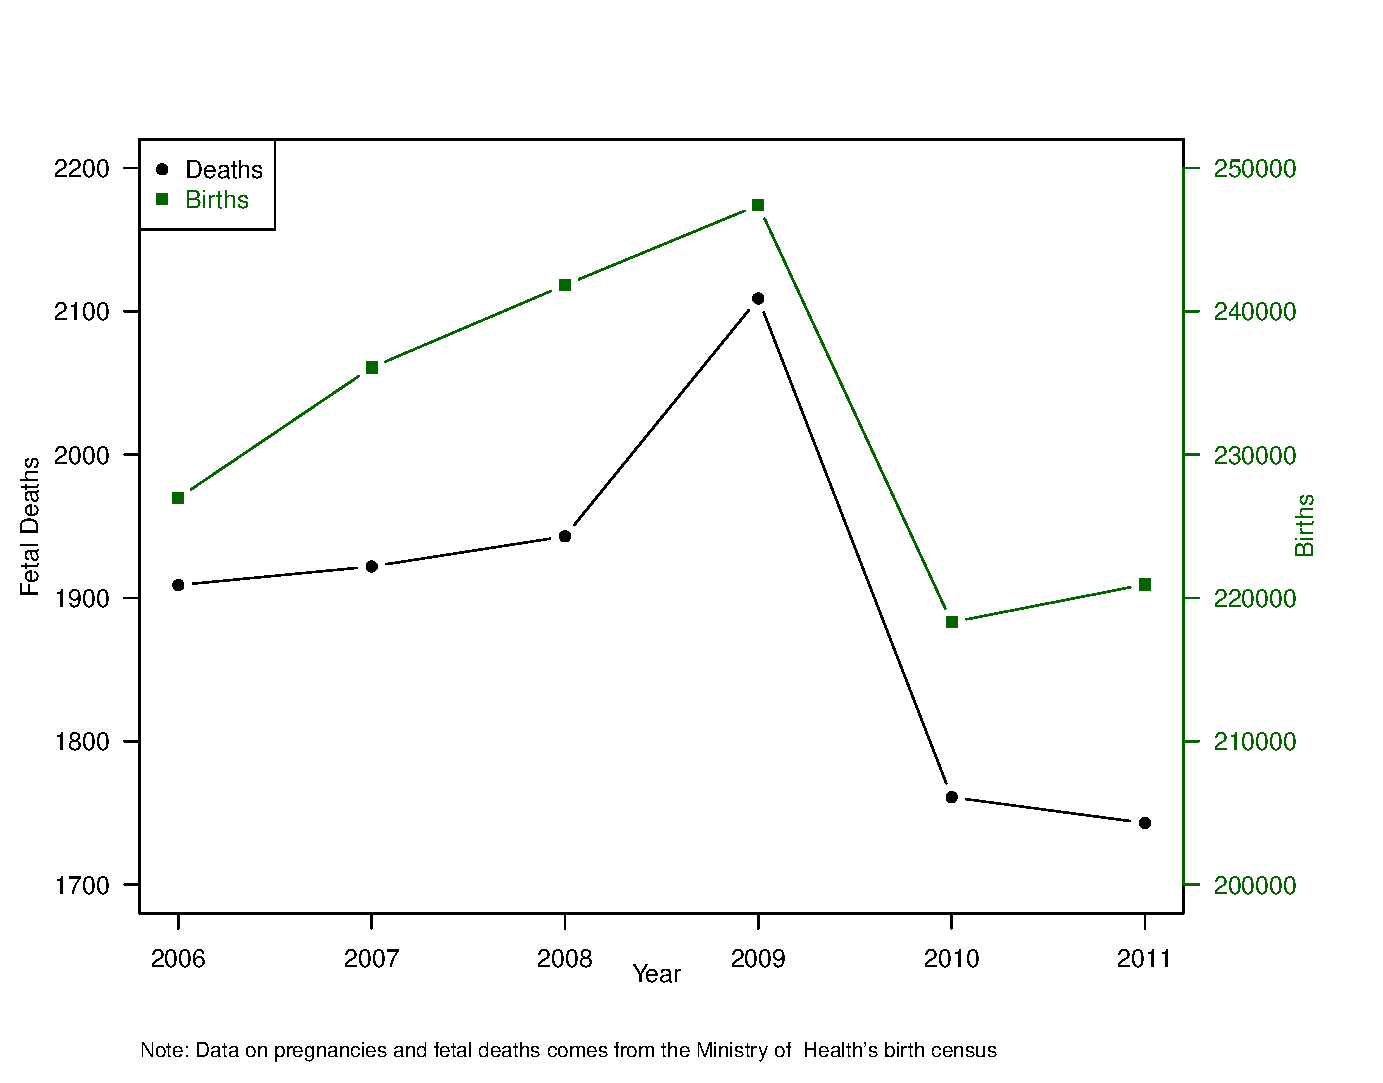
\includegraphics[scale=0.8, angle=90]{\teenfolder/Figures/BirthDeath.eps} 
%\end{center}
\end{figure}

\begin{figure}[htpb!]
\begin{center}
\caption{Pill Prescriptions and Availability by Time}
\vspace{-5mm}
\label{TEENfig:Pilltime}
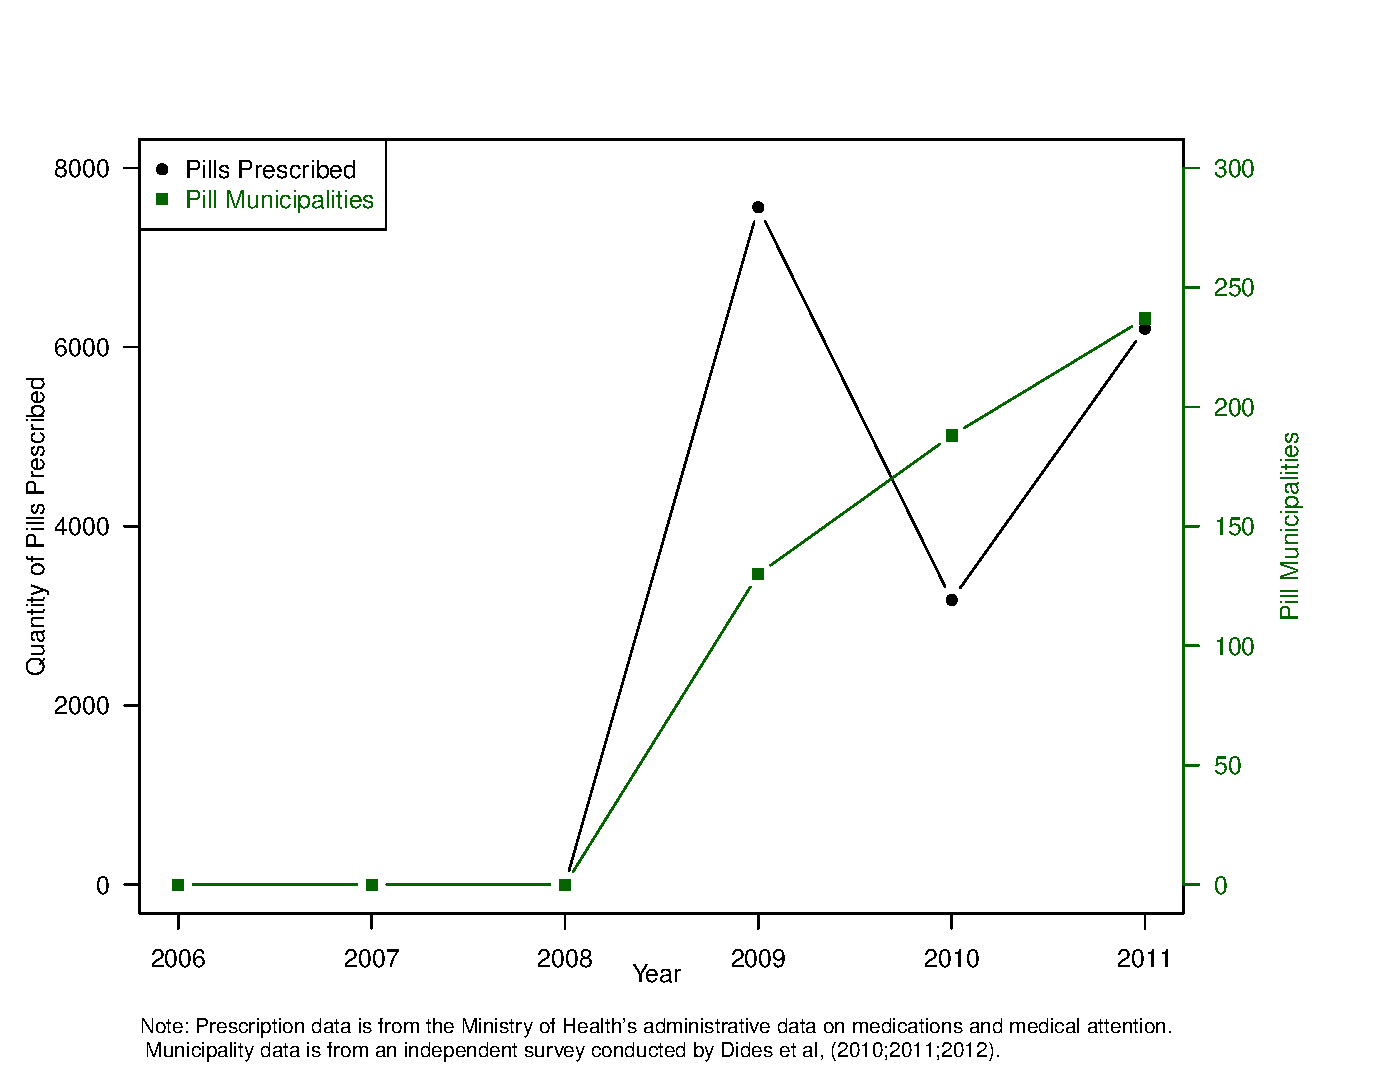
\includegraphics[scale=0.54]{\teenfolder/Figures/Pill.eps} 
\end{center}
\end{figure}

\begin{figure}[htpb!]
\begin{center}
\caption{Pregancies by Age Group and Time}
\vspace{-5mm}
\label{TEENfig:Pregtime}
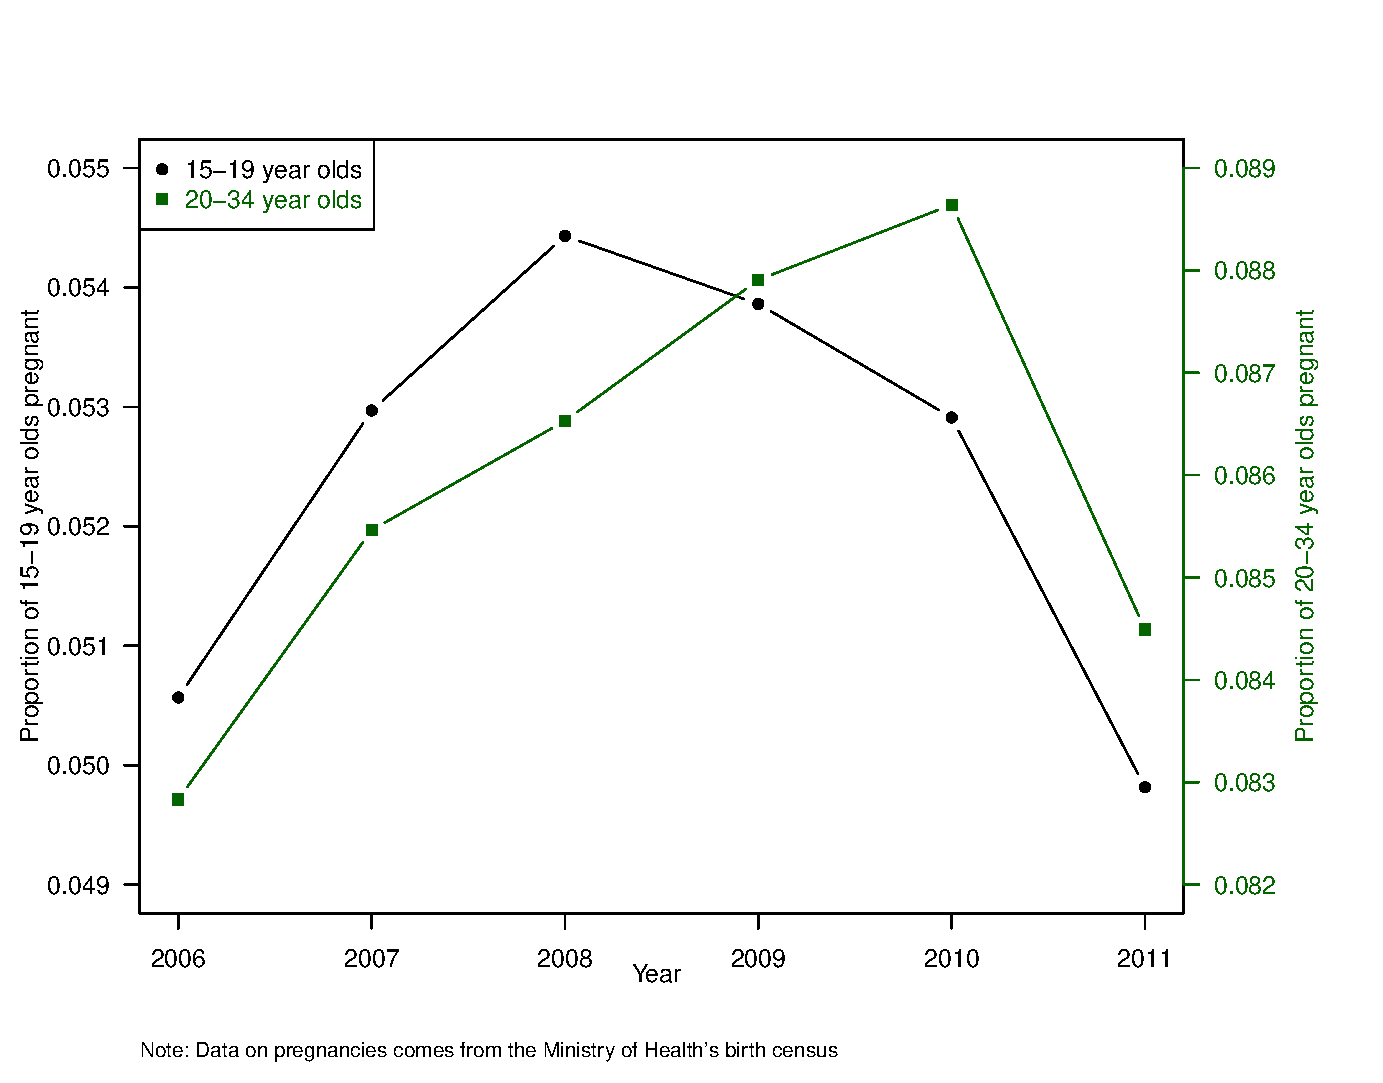
\includegraphics[scale=0.54]{\teenfolder/Figures/Births.eps} 
\end{center}
\end{figure}

\begin{figure}[htpb!]
\begin{center}
\caption{The Availability of the Pill by Geographic Region}
NOTE: THIS FIGURES HAS BEEN REMOVED TO REDUCE FILE SIZE ON github
\label{TEENfig:PillGeo}
%\includegraphics[scale=0.5]{\teenfolder/Results/Pill/Pill_l.eps} 
\end{center}
\end{figure}

\begin{figure}[htpb!]
\begin{center}
\caption{Estimates of $\hat\delta^c$ for Pregnancy (15-19)}
\label{TEENfig:Dist1519}
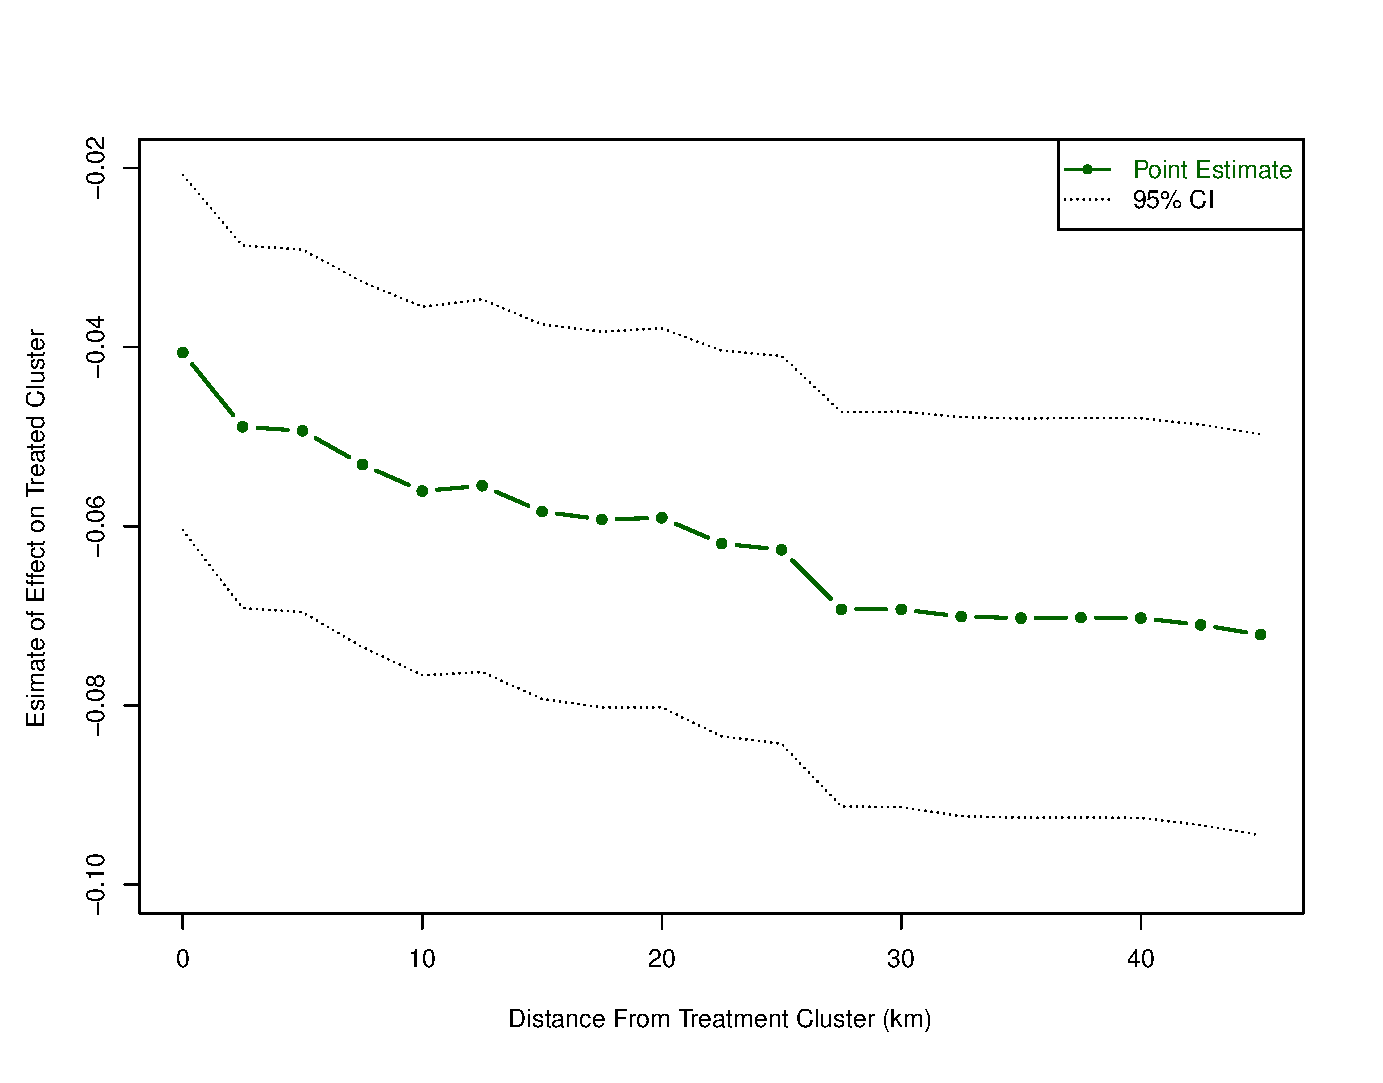
\includegraphics[scale=0.54]{\teenfolder/Figures/Dist1519.eps} 
\end{center}
\end{figure}

\begin{figure}[htpb!]
\begin{center}
\caption{Estimates of $\hat\delta^c$ for Pregnancy (20-34)}
\label{TEENfig:Dist2034}
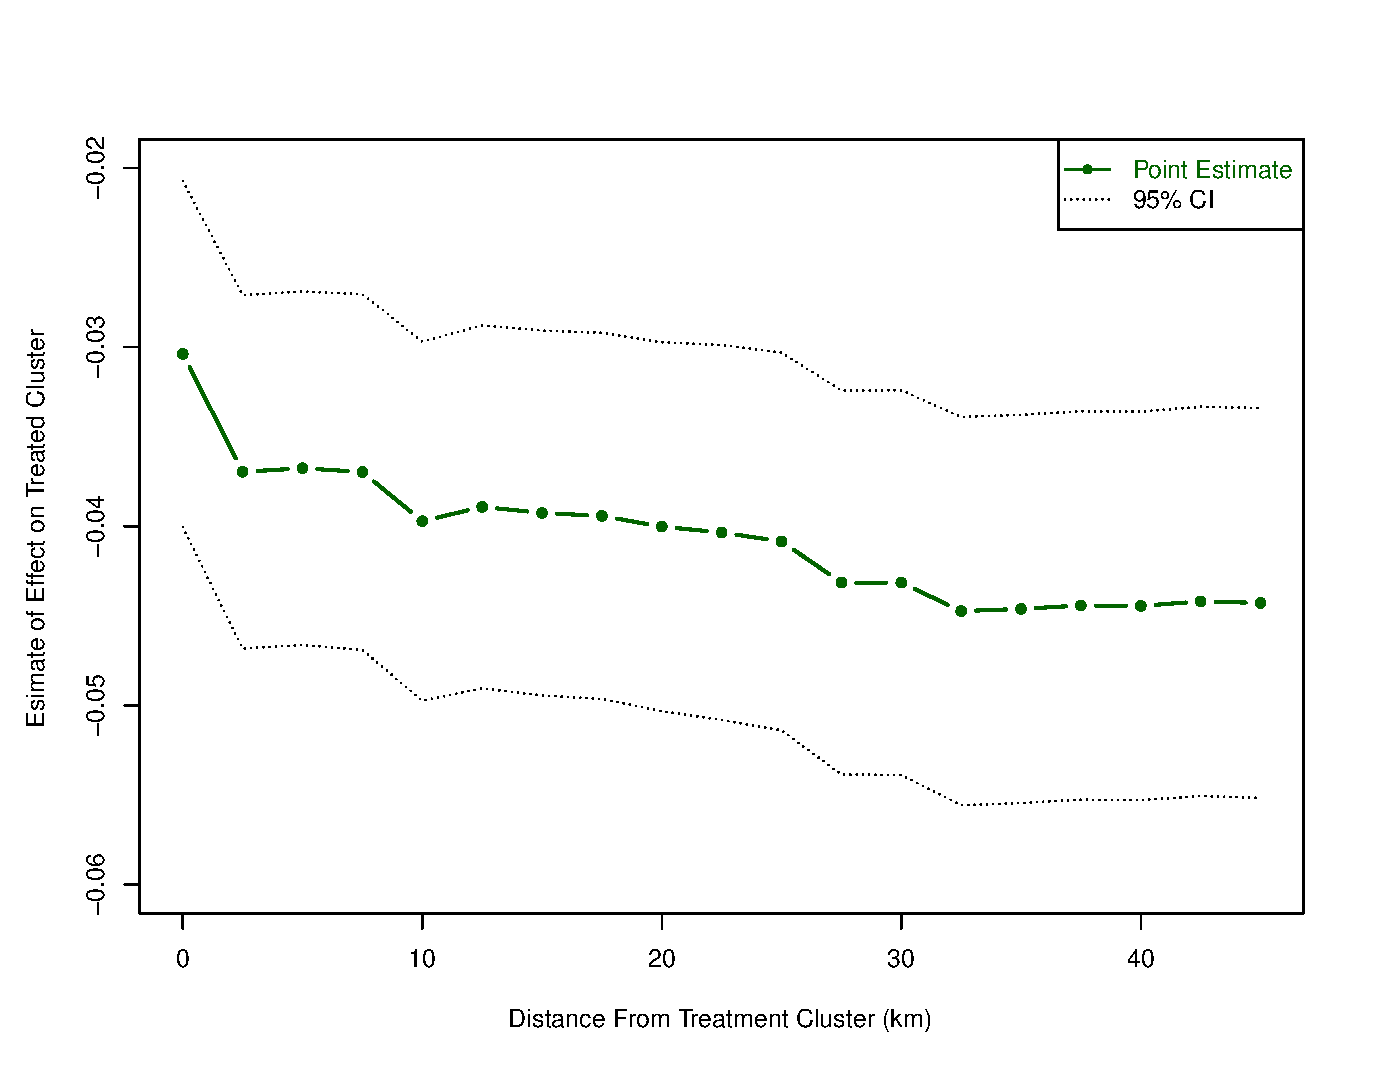
\includegraphics[scale=0.54]{\teenfolder/Figures/Dist2034.eps} 
\end{center}
\end{figure}

\clearpage

\section*{Tables}
\begin{table}[htpb!] \centering
\caption{Summary Statistics} \label{TEENtab:SumStats}
\begin{tabular} {@{\extracolsep{5pt}}lp{3mm}ccc}\\ [-1.8ex]
\hline\hline\\ [-1.8ex] &&No Pill&Pill&Total \\
&&Available&Available& \\ \midrule 
\multicolumn{5}{l}{\textbf{Municipality Characteristics}} \\
&&&& \\
Poverty &&16.4&17.0&16.6\\
&&(7.47)&(7.56)&(7.49) \\
Conservative &&0.286&0.267&0.281\\
&&(0.452)&(0.443)&(0.45) \\
Education Spending (Total) &&4,817&5,980&5,108\\
&&(5,649)&(6,216)&(5,818) \\
Education Spending (Municipal) &&430,625&525,143&454,232\\
&&(873,448)&(858,240)&(870,635) \\
Health Spending &&1,866&2,788&2,096\\
&&(2,635)&(3,381)&(2,867) \\
Out of School &&4.07&3.98&4.05\\
&&(3.16)&(3.06)&(3.13) \\
Female Mayor &&0.120&0.134&0.123\\
&&(0.325)&(0.341)&(0.329) \\
Female Poverty &&60.5&62.0&60.8\\
&&(10.64)&(9.48)&(10.4) \\
Condom Use &&0.466&0.536&0.483\\
&&(0.0506)&(0.0401)&(0.0571) \\
Pill Distance &&204&0.00&153\\
&&(5,229)&(0.00)&(4,530) \\
\multicolumn{5}{l}{\textbf{Individual Characteristics}}\\
&&&& \\
Live Births &&0.054&0.053&0.054\\
&&(0.226)&(0.224)&(0.226) \\
Fetal Deaths &&0.0558&0.0513&0.0547\\
&&(0.269)&(0.256)&(0.266) \\
Birthweight &&3322.7&3334.3&3324.7\\
&&     (540.0)&     (542.3)&     (540.4)\\
Maternal education  &&       11.92&       12.03&       11.94\\
&&     (2.967)&     (2.894)&     (2.955)\\
Percent working     &&       0.295&       0.395&       0.312\\
&&     (0.456)&     (0.489)&     (0.463)\\
Married     &&       0.340&       0.309&       0.335\\
&&     (0.474)&     (0.462)&     (0.472)\\
Age at Birth      &&       27.05&       27.15&       27.07\\
&&     (6.777)&     (6.790)&     (6.779)\\ \midrule
N Comunas &&336&280&336\\
N Fetal Deaths &&9,999&3,064&13,063\\
N Births &&1,214,088&391,212&1,605,300\\
\hline \hline \\[-1.8ex]
\multicolumn{5}{p{12cm}}{\begin{footnotesize}\textsc{Notes:}
Group means are presented with standard deviations below in
parentheses.  Poverty refers to the \% of the municipality
below the poverty line, conservative is a binary variable
indicating if the mayor comes from a politically conservative
party (UDI or RN), health and education spending are measured
 in thousands of Chilean
pesos, and pill distance measures the distance (in km) to the
nearest municipality which reports prescribing emergency
contraceptives.  Pregnancies are reported as \% of all women
giving live birth, while fetal deaths are reported per live
birth.  All summary statistics are for the period 2006-2012.
\end{footnotesize}} \normalsize\end{tabular}\end{table}


\begin{table}[!htbp] \centering
\caption{The Effect of the Morning After Pill on Pregnancy}
\label{TEENtab:PillPreg}
\scalebox{0.5}{
\begin{tabular}{@{\extracolsep{5pt}}lccccp{1mm}cccc}
\\[-1.8ex]\hline \hline \\[-1.8ex] 
&\multicolumn{4}{c}{All Births}&&\multicolumn{4}{c}{First Births}
\\ \cmidrule(r){2-5} \cmidrule(r){7-10}
&(1)&(2)&(3)&(4)&&(5)&(6)&(7)&(8)\\ \hline
\multicolumn{10}{l}{\textsc{\noindent 15-19 year olds}} \\
 & & & & & & & & & \\
Morning After Pill &$-$0.064$^{***}$&$-$0.065$^{***}$&$-$0.057$^{***}$&$-$0.057$^{***}$&&$-$0.036$^{**}$&$-$0.041$^{***}$&$-$0.031$^{**}$&$-$0.036$^{**}$\\
 &(0.015)&(0.015)&(0.015)&(0.015)&&(0.015)&(0.016)&(0.016)&(0.016)\\
 & & & & & & & & & \\
Observations&4,152,490&4,152,490&4,152,490&4,152,490&&4,125,336&4,125,336&4,125,336&4,125,336\\
McFadden's $R^2$&0.670&0.670&0.671&0.671&&0.633&0.634&0.635&0.636\\
 & & & & & & & & & \\
\multicolumn{10}{l}{\textsc{\noindent 20-34 year olds}} \\
 & & & & & & & & & \\
Morning After Pill &$-$0.040$^{***}$&$-$0.039$^{***}$&$-$0.038$^{***}$&$-$0.038$^{***}$&&$-$0.024$^{*}$&$-$0.029$^{**}$&$-$0.026$^{*}$&$-$0.029$^{**}$\\
 &(0.010)&(0.011)&(0.011)&(0.012)&&(0.014)&(0.014)&(0.015)&(0.015)\\
 & & & & & & & & & \\
Observations&11,022,111&11,022,111&11,022,111&11,022,111&&10,458,703&10,458,703&10,458,703&10,458,703\\
McFadden's $R^2$&0.772&0.772&0.773&0.773&&0.684&0.685&0.685&0.686\\
 & & & & & & & & & \\
\multicolumn{10}{l}{\textsc{\noindent 35-49 year olds}} \\
 & & & & & & & & & \\
Morning After Pill &0.001&0.001&0.005&0.008&&0.042&0.039&0.040&0.042\\
 &(0.013)&(0.013)&(0.013)&(0.013)&&(0.036)&(0.038)&(0.038)&(0.039)\\
 & & & & & & & & & \\
Observations&10,572,196&10,572,196&10,572,196&10,572,196&&10,376,895&10,376,895&10,376,895&10,376,895\\
McFadden's $R^2$&0.537&0.537&0.538&0.538&&0.641&0.641&0.642&0.642\\
\hline \\[-1.8ex] 
{\small Trends \& FEs} & Y & Y & Y & Y && Y & Y & Y & Y \\
{\small Political Controls} & & Y & Y & Y && & Y & Y & Y \\
{\small Health, Educ Controls} & & & Y & Y && & & Y & Y \\
{\small Gender Controls} & & & & Y && & & & Y \\
\hline \hline \\[-1.8ex]
\end{tabular}}\end{table}


\begin{table}[htpb!] \centering
\caption{The Effect of the Morning After Pill on Fetal Deaths}
\label{TEENtab:PillDeath}
\scalebox{0.5}{
\begin{tabular}{@{\extracolsep{5pt}}lccc}\\[-1.8ex]
\hline\hline\\[-1.8ex]
& All & Early & Late \\
& Deaths & Gestation & Gestation \\ 
& (1) & (2) & (3) \\ \midrule
\multicolumn{4}{l}{\textsc{15-19 year olds}} \\
&&&\\
Morning After Pill &$-$0.185$^{**}$&$-$0.815$^{***}$&$-$0.155\\
&(0.081)&(0.183)&(0.111)\\
&&&\\
Mean (deaths/live birth)&0.008&0.002&0.005\\
Observations&219,608&218,388&218,911\\
McFadden's $R^2$&0.232&0.378&0.251\\
&&&\\
\multicolumn{4}{l}{\textsc{20-34 year olds}} \\
&&&\\
Morning After Pill &$-$0.058&$-$0.189$^{*}$&$-$0.071\\
&(0.048)&(0.102)&(0.055)\\
&&&\\
Mean (deaths/live birth)&0.007&0.002&0.004\\
Observations&954,424&949,477&951,577\\
McFadden's $R^2$&0.198&0.385&0.170\\
&&&\\
\multicolumn{4}{l}{\textsc{35-49 year olds}} \\
&&&\\
Morning After Pill &$-$0.488$^{***}$&$-$0.776$^{***}$&$-$0.544$^{***}$\\
&(0.079)&(0.208)&(0.101)\\
&&&\\
Mean (deaths/live birth)&0.012&0.003&0.007\\
Observations&228,920&227,029&227,781\\
McFadden's $R^2$&0.260&0.411&0.238\\
\hline \hline \\[-1.8ex]
\end{tabular}}\end{table}


\begin{landscape}\begin{table}[htpb!]\centering
\caption{The EC Pill and Aggregate Human Capital} \label{TEENtab:PillAgg}
\begin{tabular}{@{\extracolsep{5pt}}lccccccccc} \\
[-1.8ex]\hline\hline \\[-1.8ex] &\multicolumn{3}{c}{15-19 year olds} &\multicolumn{3}{c}{20-34 year olds} &\multicolumn{3}{c}{35-49 year olds} \\
\cmidrule(r){2-4} \cmidrule(r){5-7} \cmidrule(r){8-10}
\textsc{Panel A:}&(1)&(2)&(3)&(4)&(5)&(6)&(7)&(8)&(9) \\
\textsc{Mother Characteristics} & Yrs Educ & Working & Married& Yrs Educ & Working & Married & Yrs Educ & Working & Married\\ \midrule
 & & & & & & & & & \\
Emergency Contraceptive Pill & 0.047&-0.003&0.000&-0.010 &-0.001& 0.006&0.028& -0.001& 0.013 \\
&[0.035]& [0.002] &[0.002]&[0.023] &[0.002] &[0.005]&[0.043] &[0.006]& [0.010] \\
 & & & & & & & & & \\
Observations & 131,605& 131,746& 131,614&896,230& 897,363& 896,318&198,885& 199,472& 198,906\\
Mean of Dep.\ Var. & 9.933 &0.023& 0.013&12.175& 0.337& 0.332&12.191& 0.531& 0.420 \\
 & & & & & & & & & \\
 & & & & & & & & & \\ \midrule
\textsc{Panel B:}&(1)&(2)&(3)&(4)&(5)&(6)&(7)&(8)&(9) \\
\textsc{Child Characteristics} & Weight & Gestation & Length& Weight & Gestation & Length & Weight & Gestation & Length\\ \midrule
 & & & & & & & & & \\
Emergency Contraceptive Pill & -4.964& -0.015& 0.009&-3.611& -0.022 &-0.025&-1.344 &-0.011& -0.037\\
& [7.539]& [0.025]& [0.029]&[3.290]& [0.018]& [0.023]&[9.169] &[0.031] &[0.037] \\
 & & & & & & & & & \\
Observations & 131,493 &131,471 &129,880&895,660 &895,671 &885,932&198,733& 198,745& 195,863\\
Mean of Dep.\ Var. & 3267.031& 38.669& 49.546&3336.382& 38.575& 49.661&3309.71& 38.236& 49.528 \\ \hline \hline \\[-1.8ex]
\multicolumn{10}{p{21.8cm}}{\begin{footnotesize}\textsc{Notes:} Each column presents an OLS regression, and full controls   listed in table \ref{TEENtab:aggregateASFR} are included.     Working and Married are binary variables, Weight is measured  in grams, Gestation in weeks, and Length in centimetres.      Summary statistics for these variables are available in table \ref{TEENtab:SumStats}.  Standard errors are clustered at the level of the municipality.$^{*}$p$<0.1$; $^{**}$p$<0.05$; $^{***}$p$<0.01$.\end{footnotesize}}
\normalsize\end{tabular}\end{table}\end{landscape}


\begin{table}[!htbp] \centering
\caption{The Morning After Pill and Treatment Spillovers}
\label{TEENtab:Spillover} 
\scalebox{0.64}{
\begin{tabular}
{@{\extracolsep{5pt}}lccc}\\[-1.8ex]\hline\hline\\
[-1.8ex] & 15-19 & 20-34 & 35-49 \\
& Year olds & Year olds & Year olds \\ \midrule
\multicolumn{4}{l}{\textsc{\noindent Panel A: Births}} \\
& & & \\
Morning After Pill &$-$0.071$^{***}$&$-$0.043$^{***}$&0.014\\
&(0.017)&(0.014)&(0.015)\\
Close $<15$ km &$-$0.077$^{***}$&$-$0.042$^{***}$&0.018\\
&(0.021)&(0.014)&(0.017)\\
Close 15-30 km &$-$0.057$^{**}$&$-$0.014&0.019\\
&(0.023)&(0.013)&(0.023)\\
Close 30-45 km &$-$0.037&$-$0.016&0.031\\
&(0.035)&(0.028)&(0.030)\\
& & & \\
Observations&4,152,490&11,022,111&7,117,890\\
McFadden's $R^2$&0.674&0.774&0.527\\ \midrule
\multicolumn{4}{l}{\textsc{\noindent Panel B: Fetal Deaths}}\\
&&&\\
Morning After Pill &$-$0.834$^{***}$&$-$0.175&$-$0.942$^{***}$\\
&(0.226)&(0.131)&(0.283)\\
Close $<15$ km &$-$0.154&$-$0.022&$-$0.200\\
&(0.235)&(0.151)&(0.240)\\
&&&\\
Observations&218,388&949,477&194,327\\
McFadden's $R^2$&0.380&0.386&0.417\\
\hline \hline \\[-1.8ex]
\multicolumn{4}{p{9.2cm}}{\begin{footnotesize}\textsc{Notes:}
$^{*}$p$<$0.1; $^{**}$p$<$0.05; $^{***}$p$<$0.01;\end{footnotesize}}
\normalsize\end{tabular}}\end{table}


\begin{landscape}
\begin{table}[!htbp] \centering
\caption{Placebo Tests}
\label{TEENtab:Placebo}
\begin{tabular}{lcccccc}
\\[-1.8ex]\hline \hline \\[-1.8ex] 
&\multicolumn{2}{c}{Lag = 3 years}
&\multicolumn{2}{c}{Lag = 4 years}
&\multicolumn{2}{c}{Lag = 5 years}
\\ \cmidrule(r){2-3} \cmidrule(r){4-5} \cmidrule(r){6-7}
&(1)&(2)&(3)&(4)&(5)&(6)\\ \hline
\textsc{Panel A: 15-19 Year-Olds} &&&&&& \\
 & & & & & & \\
Morning After Pill &0.006&$-$0.018&0.003&$-$0.004&0.006&$-$0.018\\
&(0.014)&(0.017)&(0.014)&(0.029)&(0.014)&(0.017)\\
Close $<15$ km &&$-$0.047$^{**}$&& 0.021&&0.049\\
&&(0.022)&&(0.036)&&(0.041)\\
Close 15-30 km &&$-$0.001&&$-$0.046&&0.038\\
&&(0.022)&&(0.034)&&(0.040)\\
Close 30-45 km &&$-$0.047$^{*}$&&$-$0.028&&0.089$^{**}$\\
&&(0.025)&&(0.035)&&(0.041)\\
 & & & & & & \\
Observations&4,123,049&4,123,049&4,075,854&4,075,854&4,017,339&4,017,339\\
McFadden's $R^2$&0.235&0.235&0.235&0.235&0.239&0.239\\ \midrule
\textsc{Panel A: 20-34 Year-Olds} &&&&&& \\
 & & & & & & \\
Morning After Pill &0.000& 0.002&$-$0.006& 0.006&0.000& 0.002\\
&(0.008)&(0.017)&(0.008)&(0.019)&(0.008)&(0.017)\\
Close $<15$ km && 0.008&& 0.027&&$-$0.010\\
&&(0.017)&&(0.022)&&(0.021)\\
Close 15-30 km &&$-$0.005&& 0.002&& 0.009\\
&&(0.018)&&(0.021)&&(0.019)\\
Close 30-45 km &&$-$0.001&&$-$0.004&& 0.030\\
&&(0.019)&&(0.024)&&(0.020)\\
 & & & & & & \\
Observations&10,773,289&10,773,289&10,699,388&10,699,388&10,639,773&10,639,773\\
McFadden's $R^2$&0.232&0.232&0.221&0.221&0.219&0.219\\  \hline \hline
\multicolumn{7}{p{17.2cm}}{\begin{footnotesize}\textsc{Notes:}
All specifications are identical to those estimated in tables 
\ref{TEENtab:PillPreg} and \ref{TEENtab:Spillover}.  However, 
instead of using births 1 year subsequent to the reform 
the outcome variable in each case is births and preceeding 
the reform by lag$=l\in{3,4,5}$ years, and hence entirely
unaffected in both treatment and control municipalities.
$^{*}$p$<$0.1; $^{**}$p$<$0.05; $^{***}$p$<$0.01.\end{footnotesize}}
\normalsize\end{tabular}\end{table}\end{landscape}


\newpage

\biblioinc

%\section{Appendix Tables}
%\begin{table}[!htbp] \centering
\caption{The Effect of the EC Pill on Total Births}
\label{TEENtab:aggregate}
\begin{tabular}{@{\extracolsep{5pt}}lcccc}
\\[-1.8ex]\hline \hline \\[-1.8ex] 
& Number& Number & Number & Number \\
& Births& Births & Births & Births \\
&(1)&(2)&(3)&(4) \\ \hline
\multicolumn{5}{l}{\textbf{
\noindent Panel A: All Women}} \\
Emergency Contraceptive Pill&7.623&$-$27.564$^{***}$&$-$20.337$^{***}$&$-$25.936$^{***}$\\
            &[5.720]&[5.242]&[5.954]&[8.511]\\
 & & & & \\
Observations&2,210&2,210&2,210&2,210\\
Mean Number of Births&2632.67&2632.67&2632.67&2632.67\\
 & & & & \\
\multicolumn{5}{l}{\noindent \textbf{
Panel B: 15-19 year olds}} \\
Emergency Contraceptive Pill&$-$8.618$^{***}$&$-$8.519$^{***}$&$-$5.583$^{***}$&$-$7.474$^{***}$\\
            &[1.233]&[1.517]&[1.716]&[2.275]\\
 & & & & \\
Observations&2,205&2,205&2,205&2,205\\
Mean Number of Births&386.14&386.14&386.14&386.14\\
 & & & & \\
\multicolumn{5}{l}{\noindent \textbf{
Panel C: 20-34 year olds}} \\
Emergency Contraceptive Pill&11.605$^{***}$&$-$16.644$^{***}$&$-$12.890$^{***}$&$-$17.893$^{***}$\\
            &[4.173]&[3.621]&[4.257]&[6.101]\\
 & & & & \\
Observations&2,210&2,210&2,210&2,210\\
Mean Number of Births&1833.11&1833.11&1833.11&1833.11\\
 & & & & \\
\multicolumn{5}{l}{\noindent \textbf{
Panel B: 35-49 year olds}} \\
Emergency Contraceptive Pill&4.636$^{***}$&$-$2.401$^{*}$&$-$1.843&$-$0.541\\
            &[1.608]&[1.299]&[1.371]&[1.742]\\
 & & & & \\
Observations&2,210&2,210&2,210&2,210\\
Mean Number of Births&435.78&435.78&435.78&435.78\\
\hline \\[-1.8ex] 
{\small Year \& Comuna FEs}             &Y&Y&Y&Y \\
{\small Municipal-Specific Linear Trends}& &Y&Y&Y \\
{\small Time Varying Controls}           & & &Y&Y \\
{\small Spillovers}                      & & & &Y \\
\hline \hline \\[-1.8ex]
\multicolumn{5}{p{14.2cm}}{\begin{footnotesize}
\textsc{Notes:} Each panel presents population       
weighted difference-in-difference results for a       
regression of the total number of births for the age  
group in each municipality. Specifications are        
identical to table \ref{TEENtab:aggregateASFR},      
however birth weights are replaced by the total number
 of births. Standard errors are clustered             
at the level of the municipality.
$^{*}$p$<$0.1; $^{**}$p$<$0.05; $^{***}$p$<$0.01\end{footnotesize}}
\normalsize\end{tabular}\end{table}

\begin{table}[!htbp] \centering
\caption{The Effect of the EC Pill on Birth Rates}
\label{TEENtab:aggregateASFR}
\begin{tabular}{@{\extracolsep{5pt}}lcccc}
\\[-1.8ex]\hline \hline \\[-1.8ex] 
& Birth& Birth& Birth& Birth\\
& Rate & Rate & Rate & Rate \\
&(1)&(2)&(3)&(4) \\ \hline
\multicolumn{5}{l}{\textbf{
\noindent Panel A: All Women}} \\
Emergency Contraceptive Pill     &$-$1.193$^{***}$&$-$2.247$^{***}$&$-$1.562$^{***}$&$-$1.721$^{***}$\\
            &[0.425]&[0.489]&[0.524]&[0.620]\\
 & & & & \\
Observations&2,210&2,210&2,210&2,210\\
Mean Birth Rate&53.87&53.87&53.87&53.87\\
 & & & & \\
\multicolumn{5}{l}{\noindent \textbf{
Panel B: 15-19 year olds}} \\
Emergency Contraceptive Pill&$-$3.811$^{***}$&$-$4.546$^{***}$&$-$2.795$^{**}$&$-$3.536$^{**}$\\
            &[0.714]&[1.179]&[1.218]&[1.538]\\
 & & & & \\
Observations&2,205&2,205&2,205&2,205\\
Mean Birth Rate&52.00&52.00&52.00&52.00\\
 & & & & \\
\multicolumn{5}{l}{\noindent \textbf{
Panel C: 20-34 year olds}} \\
Emergency Contraceptive Pill&$-$2.491$^{***}$&$-$3.277$^{***}$&$-$2.273$^{**}$&$-$2.452$^{**}$\\
            &[0.762]&[0.891]&[0.938]&[1.116]\\
 & & & & \\
Observations&2,210&2,210&2,210&2,210\\
Mean Birth Rate&85.49&85.49&85.49&85.49\\
 & & & & \\
\multicolumn{5}{l}{\noindent \textbf{
Panel B: 35-49 year olds}} \\
Emergency Contraceptive Pill&0.240&$-$0.586&$-$0.401&$-$0.106\\
            &[0.274]&[0.411]&[0.455]&[0.600]\\
 & & & & \\
Observations&2,210&2,210&2,210&2,210\\
Mean Birth Rate&21.40&21.40&21.40&21.40\\
\hline \\[-1.8ex] 
{\small Year \& Comuna FEs}             &Y&Y&Y&Y \\
{\small Municipal-Specific Linear Trends}& &Y&Y&Y \\
{\small Time Varying Controls}           & & &Y&Y \\
{\small Spillovers}                      & & & &Y \\
\hline \hline \\[-1.8ex]
\multicolumn{5}{p{12.8cm}}{\begin{footnotesize}
\textsc{Notes:} Each panel presents population-weighted
 difference-in-difference results for a regression of 
age-specific fertility rates (ASFR) on the EC reform for
 the age group in
 each municipality.  ASFR is defined as the number of   
births per 1,000 women.  In the case of all women, this 
is called the General Fertility Rate (GFR). All models  
are estimated by OLS, and each municipality is          
weighted by the population of women. Time varying       
controls included in the regression consist of party    
dummies for the mayor in power, the mayor's gender, the
 vote margin of the mayor, the percent of girls out of  
highschool, education spending spending by both the     
municipality and the Ministry of Education, total       
health spending and health spending on staff and        
training, the percent of female heads of households     
living below the poverty line, the percent of female    
workers in professional positions in the Municipality,  
and condom availability (measured at the level of the   
region). Standard errors are clustered at the level of  
the municipality.
$^{*}$p$<$0.1; $^{**}$p$<$0.05; $^{***}$p$<$0.01\end{footnotesize}}
\normalsize\end{tabular}\end{table}


%\begin{table}[htpb!] \centering 
  \caption{The Morning After Pill and Pregnancy: Full Covariates} 
  \label{TEENtabPregFull} 
\begin{tabular}{@{\extracolsep{5pt}}lccc} 
\\[-1.8ex]\hline 
\hline \\[-1.8ex] 
 & \multicolumn{3}{c}{Pregnancy} \\ 
\cline{2-4} 
\\[-1.8ex] & 15-19 & 20-34 & 35-49 \\ 
 & year olds & year olds & year olds \\ 
\\[-1.8ex] & \multicolumn{1}{c}{(1)} & \multicolumn{1}{c}{(2)} & \multicolumn{1}{c}{(3)}\\ 
\hline \\[-1.8ex] 

 Morning After Pill & -0.041$^{***}$ & -0.030$^{***}$ & 0.006 \\ 
  & (0.010) & (0.005) & (0.010) \\ 
  & & & \\ 
 Female Mayor & 0.016 & -0.005 & -0.007 \\ 
  & (0.026) & (0.013) & (0.026) \\ 
  & & & \\ 
 Mayor's Support & 0.054 & 0.017 & -0.129 \\ 
  & (0.084) & (0.042) & (0.085) \\ 
  & & & \\ 
 Out of School & -0.004 & -0.001 & -0.001 \\ 
  & (0.003) & (0.001) & (0.003) \\ 
  & & & \\ 
 Total Education Spending & 0.001$^{*}$ & -0.00004 & 0.001$^{**}$ \\ 
  & (0.0003) & (0.0002) & (0.0003) \\ 
  & & & \\ 
 Municipal Education Spending & -0.004$^{***}$ & -0.001$^{**}$ & -0.001$^{**}$ \\ 
  & (0.001) & (0.0003) & (0.001) \\ 
  & & & \\ 
 Health Spending & -0.0002 & 0.0001 & -0.0005 \\ 
  & (0.001) & (0.0003) & (0.001) \\ 
  & & & \\ 
 Health Training & -0.080$^{***}$ & -0.036$^{***}$ & 0.005 \\ 
  & (0.024) & (0.012) & (0.025) \\ 
  & & & \\ 
 Health Staff & 0.001 & 0.001$^{***}$ & -0.0004 \\ 
  & (0.001) & (0.0005) & (0.001) \\ 
  & & & \\ 
 Female Poverty & -0.0004 & -0.0001 & 0.002$^{***}$ \\ 
  & (0.001) & (0.0003) & (0.001) \\ 
  & & & \\ 
 Female Workers & -0.001 & -0.0005 & 0.001 \\ 
  & (0.001) & (0.0004) & (0.001) \\ 
  & & & \\ 
\hline \\[-1.8ex] 
Years $\times$ Municipality & 1,929 & 1,934 & 1,934 \\ 
\hline 
\hline \\[-1.8ex] 
\multicolumn{4}{p{10.8cm}}{\begin{footnotesize} \textsc{Notes:} Each model is identical to 
            column (4) of table \ref{TEENtab:PillPreg}.  A description of each 
            variable is also provided in table \ref{TEENtab:PillPreg}.  Municipality
            dummies and trends and political party dummies have been omitted for 
            clarity. $^{*}$p$<$0.1; $^{**}$p$<$0.05; $^{***}$p$<$0.01 
            \end{footnotesize}} \\ 
\end{tabular} 
\end{table} 


%\begin{table}[htpb!] \centering 
  \caption{The Morning After Pill and Fetal Death: Full Covariates} 
  \label{TEENtabDeathFull} 
\begin{tabular}{@{\extracolsep{5pt}}lccc} 
\\[-1.8ex]\hline 
\hline \\[-1.8ex] 
 & \multicolumn{3}{c}{Fetal Death (0-20 Weeks)} \\ 
\cline{2-4} 
\\[-1.8ex] & 15-19 & 20-34 & 35-49 \\ 
 & year olds & year olds & year olds \\ 
\\[-1.8ex] & \multicolumn{1}{c}{(1)} & \multicolumn{1}{c}{(2)} & \multicolumn{1}{c}{(3)}\\ 
\hline \\[-1.8ex] 
 Morning After Pill & -0.815$^{***}$ & -0.189$^{*}$ & -0.776$^{***}$ \\ 
  & (0.237) & (0.113) & (0.217) \\ 
  & & & \\ 
  Female Mayor & 0.987$^{*}$ & 0.096 & -0.270 \\ 
  & (0.593) & (0.293) & (0.528) \\ 
  & & & \\ 
  Mayor's Support & 1.861 & 1.168 & -0.416 \\ 
  & (1.886) & (0.989) & (1.783) \\ 
  & & & \\ 
  Out of School & -0.005 & -0.003 & 0.074 \\ 
  & (0.083) & (0.032) & (0.064) \\ 
  & & & \\ 
  Total Education Spending & 0.0001 & -0.00003 & -0.00003 \\ 
  & (0.0001) & (0.00004) & (0.0001) \\ 
  & & & \\ 
  Municipal Education Spending & 0.0004$^{*}$ & 0.0001 & 0.0001 \\ 
  & (0.0002) & (0.0001) & (0.0001) \\ 
  & & & \\ 
  Health Spending & -0.0001 & 0.0002$^{**}$ & 0.0001 \\ 
  & (0.0002) & (0.0001) & (0.0001) \\ 
  & & & \\ 
  Health Training & 0.005 & -0.003 & 0.005 \\ 
  & (0.004) & (0.002) & (0.004) \\ 
  & & & \\ 
  Health Staff & 0.00004 & 0.00004 & 0.0001 \\ 
  & (0.0002) & (0.0001) & (0.0002) \\ 
  & & & \\ 
  Female Poverty & 0.017 & 0.002 & 0.002 \\ 
  & (0.016) & (0.007) & (0.013) \\ 
  & & & \\ 
  Female Workers & 0.008 & -0.006 & 0.018 \\ 
  & (0.019) & (0.008) & (0.014) \\ 
  & & & \\ 
 \hline \\[-1.8ex] 
Years $\times$ Municipality & \multicolumn{1}{c}{1,887} & \multicolumn{1}{c}{1,912} & \multicolumn{1}{c}{1,891} \\ 
Akaike Inf. Crit. & \multicolumn{1}{c}{2,594.943} & \multicolumn{1}{c}{4,244.940} & \multicolumn{1}{c}{2,811.065} \\ 
\hline 
\hline \\[-1.8ex] 
\multicolumn{4}{p{10.8cm}}{\begin{footnotesize} \textsc{Notes:} Each model is identical to 
          column (2) of table \ref{TEENtab:PillDeath}.  A description of each 
          variable is also provided in table \ref{TEENtab:PillPreg}.  Municipality
          dummies and trends and political party dummies have been omitted for 
          clarity. $^{*}$p$<$0.1; $^{**}$p$<$0.05; $^{***}$p$<$0.01 
          \end{footnotesize}} \\ 
\normalsize 
\end{tabular} 
\end{table} 



\begin{table}[!htbp] \centering
\caption{Back of the Envelope Calculation of Effect Sizes}
\label{TEENtab:BOE}
\begin{tabular}{@{\extracolsep{5pt}}lcc}
\\[-1.8ex]\hline \hline \\[-1.8ex] 
& 18 \& Under & 19 \& Over\\ 
&(1)&(2) \\ \hline
 & &  \\
Morning After Pill &$-$0.069$^{***}$&$-$0.032$^{***}$\\
&(0.019)&(0.010)\\
Close $<15$ km &$-$0.075$^{***}$&$-$0.032$^{***}$\\
&(0.026)&(0.012)\\
Close 15-30 km &$-$0.049$^{*}$&$-$0.013\\
&(0.028)&(0.012)\\
& & \\ \midrule
N Preg (pill) &20,713&172,557\\
N Preg (close 15) &10,370&100,749\\
N Preg (close 30) &6,141&48,756\\
Pills Disbursed & 5,736 & 11,121 \\
\hline \hline \\[-1.8ex]
\multicolumn{3}{p{7.2cm}}{\begin{footnotesize}\textsc{Notes:} 
Regression coefficients and standard errors are calculated in 
line with specification (\ref{TEENeqn:spillover}). The number of 
pills disbursed is calculated from administrative data described in 
figure \ref{TEENfig:Pilltime}, and number of avoided pregnancy is 
based on regression estimates and total births in administrative 
data. Further details are provided in appendix \ref{TEENscn:BOE}.
$^{*}$p$<$0.1; $^{**}$p$<$0.05; $^{***}$p$<$0.01\end{footnotesize}}
\normalsize\end{tabular}\end{table}







%\appendix
%\section*{Online Appendix}
%\section{Data Agreement with Government of Chile}
%\includepdf[pages={-}]{\teenfolder/Data/DECLARACION_CONFIDENCIALIDAD.pdf}


\end{spacing}
\end{document}
